% ERRORQUAKE — NeurIPS 2026 Evaluations & Datasets track submission.
% Double-blind. Every number in this paper comes from a JSON file in
% results/analysis/*.json — do not invent, round, or approximate.

\documentclass{article}
\usepackage[eandd]{neurips_2026}
\usepackage[utf8]{inputenc}
\usepackage[T1]{fontenc}
\usepackage{microtype}
\usepackage{amsmath,amssymb,amsthm}
\usepackage{booktabs}
\usepackage{graphicx}
\usepackage{xcolor}
\usepackage{array}
\usepackage{hyperref}
\usepackage{cleveref}
\usepackage{natbib}

\graphicspath{{figs/}}

% Short-hand macros (used consistently throughout the paper).
% \sdi expands to "b" — works inside or outside math mode via \ensuremath.
\newcommand{\sdi}{\ensuremath{b}}
\newcommand{\bvalue}{severity distribution index (\sdi)}

\title{ERRORQUAKE: Heavy-Tailed Error Severity Distributions\\
in Open-Weight Large Language Models}

\author{Anonymous submission}

\begin{document}
\maketitle

% =====================================================================
\begin{abstract}
\textbf{Larger dense open-weight LLMs concentrate their remaining
errors in the upper tail.} Hallucination benchmarks report a scalar
error rate and treat all errors as equivalent. We introduce
\textsc{Errorquake-4k}, a $4{,}000$-query benchmark that scores each
response on a continuous $0$--$4$ severity scale across $8$ domains
and $5$ difficulty tiers, and we fit per-model severity distributions
for $21$ open-weight models spanning $3$B to $37$B active parameters.
For each model we estimate a \textbf{severity distribution index}
(\sdi{}, the Gutenberg--Richter slope) on the upper tail. Across the
$14$ dense models, $\rho_s(\log_{10}\mathrm{params},\,\sdi) = -0.689$
($p = 0.006$, leave-one-out robust): larger dense models are more
accurate but their upper-tail slopes are shallower. The sign is
specific to the upper-tail estimator; under fixed $m_{\min}$ that
fits the bulk of the positive grid, the sign flips
($\rho_s = +0.84$), indicating that larger dense models commit
fewer small errors but a relatively higher fraction of catastrophic
ones. Three supporting results. \emph{First}, severity distributions
exhibit tail structure beyond exponential decay: $17/21$ have a
non-exponential best fit by BIC, $18/21$ Vuong-decisive
($p<0.05$); families are stretched exponential (10), truncated
power law (5), exponential (4), lognormal (2). \emph{Second}, the
\sdi{} adds information beyond accuracy: $30/210$ pairs have
disjoint $95\%$ \sdi{} CIs at matched accuracy
($|\Delta\varepsilon|<0.05$), e.g.\ \textsc{deepseek-v3.2} vs.\
\textsc{ministral-14b} at $\varepsilon=0.586$ and $\Delta\sdi=0.47$.
\emph{Third}, micro-error \sdi{} on easy queries rank-orders
catastrophic counts on hard queries at $\rho=0.44$ ($p=0.044$),
failing the pre-registered $\rho \geq 0.75$ threshold for calibrated
absolute-rate prediction. Accuracy and tail shape are correlated
($\rho_s(\varepsilon, \sdi) = -0.73$ on dense), but \sdi{} provides
discriminative information \emph{beyond} accuracy and should be
reported alongside it.
\end{abstract}

% =====================================================================
\section{Introduction}\label{sec:intro}

Standard hallucination benchmarks
\citep{lin2022truthfulqa,liu2023halueval} report a single number ---
the error rate $\varepsilon$ --- and treat all errors as equivalent.
This collapses a fundamental property of language model failure: an
LLM that cites the wrong publication date and an LLM that fabricates
an entire judicial opinion both contribute one count to $\varepsilon$,
yet their downstream consequences differ by orders of magnitude.
The question that matters in deployment is not ``how often does the
model err?'' but ``how badly?''. Borrowing the vocabulary of
seismology, we summarise an LLM's tail behaviour with the slope $b$
of the Gutenberg--Richter magnitude-frequency relation
$\log_{10} N(M \geq m) = a - b\,m$: small $b$ means the model emits
few errors but the rare ones are catastrophic; large $b$ means many
small errors with bounded severity.

\paragraph{Central finding and evaluative role.}
\emph{The severity distribution of an LLM's errors carries
discriminative information beyond the error rate, and the upper-tail
slope varies systematically with model scale.} On the $14$ dense
open-weight models in our catalog, the upper-tail \bvalue{}
anti-correlates with $\log_{10}$(active params) at
$\rho_s = -0.689$ ($p = 0.006$, leave-one-out robust in
$14/14$ drops). The marginal correlation is partly mediated by
accuracy --- in our catalog, larger dense models also have higher
error rates ($\rho_s(\log_{10}\text{params},\,\varepsilon) = +0.59$),
and $\varepsilon$ and \sdi{} themselves correlate
($\rho_s = -0.73$). At matched accuracy ($|\Delta\varepsilon| <
0.05$), $30/210$ model pairs in our catalog have disjoint
\sdi{} confidence intervals --- direct evidence that \sdi{} is
not redundant with $\varepsilon$. \emph{Accuracy and severity
distribution should be reported together; \sdi{} discriminates
models that the error rate treats as equivalent.} This paper
contributes to AI evaluation by introducing severity distribution
analysis as a complementary axis to accuracy-based evaluation,
under the assumption that error severity can be reliably scored on
a continuous scale by a dual-judge pipeline. The claim applies to
open-weight instruction-tuned models at $3$--$37$B active
parameters; it does not yet cover proprietary frontier models,
reasoning models, or models below $3$B
(\S\ref{sec:limitations}). The benchmark, scoring pipeline, scale
anchors, and analysis code are released for replication.

\paragraph{Contributions.}
\textbf{C1} A continuous 9-point error-severity scale with
anchors, a dual-judge scoring pipeline, and a $340$-item human
calibration set (\S\ref{sec:method}, Appendix~\ref{app:scale}).
\textbf{C2} \textsc{Errorquake-4k}: $4{,}000$ queries $\times$ $21$
open-weight models with per-model severity distributions.
\textbf{C3} Distribution characterisation: $18/21$ Vuong-decisive,
no pure power laws (\S\ref{sec:exp1}).
\textbf{C4} \sdi{} as model discriminator: $30$ pairs with
disjoint CIs at matched accuracy (\S\ref{sec:exp2}).
\textbf{C5 (headline)} Negative scaling correlation in dense
models: $\rho_s = -0.689$ ($p = 0.006$, $n_{\text{dense}} = 14$,
LOO-robust) --- larger dense models have heavier severity tails
(\S\ref{sec:exp5}).
\textbf{C6} Pre-registered micro-error prediction: moderate
rank signal ($\rho_s = 0.44$, $p = 0.044$), absolute-rate
prediction fails; the failure is a difficulty-tier level shift,
not a slope divergence (\S\ref{sec:exp3}).

% =====================================================================
\section{Related Work}\label{sec:related}

\paragraph{Hallucination benchmarks.} \textsc{TruthfulQA}
\citep{lin2022truthfulqa}, \textsc{HaluEval} \citep{liu2023halueval},
\textsc{FaithDial} \citep{dziri2024faithdial}, and the
\citet{ji2023survey} survey establish the dominant evaluation
protocol for LLM factuality: a held-out question set, a binary
correctness label per response, and an aggregate error rate per
model. None of these reports a severity distribution. The tacit
assumption is that all errors are exchangeable, so that reducing
the count is sufficient to reduce the risk. We show empirically
that the same accuracy can hide an order-of-magnitude gap in
catastrophic event rate (\S\ref{sec:exp2}), and that scaling
\emph{worsens} the severity profile of the residual errors
(\S\ref{sec:exp5}); the standard protocol misses both effects.

\paragraph{Error severity in NLP (positioning against
\citet{asgari2025severity}).} \citet{asgari2025severity} score
hallucinations on a three-bin scale (minor / moderate / severe) and
report per-model severity histograms, arguing that the distribution
of severities is informative beyond the aggregate rate. Our
contribution differs along three axes. \emph{First}, we use a
$9$-level continuous scale quantised at $0.5$ increments, not three
ordinal bins, and show (sensitivity S1, \S\ref{sec:sensitivity})
that coarse scales destroy the discriminative power of the
distribution index. \emph{Second}, we fit parametric distribution
families and report a single summary statistic (the \sdi{})
anchored to the Gutenberg--Richter magnitude-frequency relation,
which enables quantitative cross-model comparison and
between-regime extrapolation that histogram-only methods cannot
support. \emph{Third}, we cover $21$ models spanning an order of
magnitude in active parameters, which is what enables the headline
negative scaling correlation; prior severity-focused work evaluates
on only a few models. We are, to our knowledge, the first to
report a severity-distribution-vs-scale anti-correlation on a
multi-model benchmark.

\paragraph{Calibration and uncertainty quantification.}
\citet{guo2017calibration} show modern neural classifiers are
overconfident; \citet{lin2022teaching} and \citet{kadavath2022language}
explore whether LLMs can verbalise their own uncertainty. These
works are concerned with the \emph{confidence} side of the calibration
problem --- does the model know when it is wrong? --- while our
contribution is on the \emph{severity} side: when the model is
wrong, how badly wrong, and does that badness follow a law. The
two axes are orthogonal and complementary: a well-calibrated model
could still have a heavy severity tail, and a poorly calibrated
model could still have a light one.

\paragraph{Heavy-tailed phenomena in machine learning.}
\citet{taleb2020statistical} provides the statistical vocabulary
for heavy-tailed distributions and power-law diagnostics that we
borrow. In neural network training, heavy tails appear in
gradient-norm distributions and loss landscapes, but these are
distinct objects from the error severity distribution we study.
\citet{clauset2009power} supply the standard maximum-likelihood
power-law-fitting recipe; we follow their protocol with a
discreteness correction appropriate to a 9-level ordinal severity
scale.

\paragraph{Scaling laws.} Language model accuracy scales with
compute and parameter count
\citep{kaplan2020scaling,hoffmann2022chinchilla,wei2022emergent};
mixture-of-experts architectures decouple active from total
parameters \citep{fedus2022moe}. These laws describe how often
models are wrong. Our contribution is orthogonal: we ask how
\emph{badly} models are wrong as a function of scale, and we
document a relationship that moves in the opposite direction from
the accuracy scaling law in the dense subset of the open-weight
ecosystem.

\paragraph{Severity-aware evaluation in the broader landscape.}
Hallucination taxonomies and long-tail-knowledge surveys
\citep{ji2023survey} argue qualitatively that tail events --- rare
but high-consequence failures --- are where deployment harms
concentrate, and that binary accuracy obscures this risk
heterogeneity. Our work operationalises that concern: rather than
arguing in prose that tails matter, we fit distributional models to
error severity and extract a quantitative index (\sdi) that makes
the tail shape comparable across models.

\paragraph{Calibration as a related axis.} Uncertainty calibration
and severity distribution are conceptually distinct but empirically
correlated axes of model quality. A well-calibrated model that
expresses appropriate uncertainty may still have a heavy severity
tail when it does err confidently; conversely, a poorly calibrated
model may have a light tail. Work on confidence calibration
\citep{guo2017calibration,kadavath2022language} complements our
contribution: combining the two axes would identify models that
are both calibrated and tail-light --- the safest deployment
profile. We document the empirical correlation between accuracy
and tail shape on our catalog in \S\ref{sec:exp5}.

\paragraph{Concurrent severity-aware and domain-specific
hallucination benchmarks.} Several recent works evaluate
hallucination in specific domains or modalities:
\citet{dahl2024hallucination} decomposes domain-specific
hallucination types in legal LLMs; \citet{cliniqlink2024},
\citet{medheval2024}, \citet{medhallbench2024}, and
\citet{medhallu2024} target medical and clinical factuality;
\citet{hallucinogen2024} extends hallucination evaluation to
vision-language models; and \citet{her2024speech} addresses speech.
\citet{halueval2024v2} updates the original HaluEval benchmark
with stricter type taxonomies. These works share our premise that
binary accuracy obscures critical failure modes, but focus on
finer-grained type taxonomies within a single domain or modality.
\textsc{Errorquake} is complementary: we model the severity
\emph{distribution} across eight general domains and extract a
quantitative tail index that enables cross-model comparison and
scaling-law analysis --- capabilities that domain-specific
taxonomies, by design, do not provide.

% =====================================================================
\section{Method}\label{sec:method}

\paragraph{Error-severity scale.} We score each model response on
a continuous $0.0$--$4.0$ scale quantised to $0.5$ increments
($9$ distinct levels). $0.0$ denotes a correct response;
$0.5$--$1.0$ mark imprecisions that preserve the gist; $1.5$--$2.0$
denote moderate factual errors; $2.5$--$3.0$ denote substantial
errors that mislead a typical reader; $3.5$--$4.0$ denote
fabrication (confident assertion of invented information).
Appendix~\ref{app:scale} reproduces the full rubric with three
worked examples per anchor. Scale design principles:
(i) continuous, not binary; (ii) non-negative; (iii) dense near
the ``harmless slip vs consequential failure'' boundary.

\paragraph{Query benchmark.} \textsc{Errorquake-4k} comprises
$4{,}000$ queries: $500$ per domain across $8$ domains (BIO, LAW,
HIST, GEO, SCI, TECH, FIN, CULT), with each domain stratified into
five difficulty tiers T1--T5 of $100$ queries each. Tiers T1--T2
are ``easy'' factual queries; T4--T5 contain trap questions and
compositional lookups designed to elicit confident fabrication.
A tier-calibration audit flagged ${\sim}6\%$ of cells as mis-tiered
and these were regenerated (Appendix~\ref{app:benchmark}).

\paragraph{Dual-judge scoring.} Each response is scored by two
judges from an $8$-model round-robin pool that excludes the target
model (zero self-judging, audited). Final score = mean of the two
judges when they agree within $1.0$; otherwise median-of-three with
a tiebreaker. Pre-tiebreak inter-judge agreement on the $60{,}568$
records where both judges produced a score is
$\mathrm{ICC}(2,1) = 0.374$ (single-rater, two-way random effects,
absolute agreement; Shrout--Fleiss). \emph{The averaged final score
that the paper actually uses has $\mathrm{ICC}(2,k{=}2) = 0.545$,}
in the ``fair--moderate'' range of Cicchetti's guidelines, and is
the relevant reliability number for downstream analyses. Linear
Cohen's $\kappa = 0.285$ and quadratic $\kappa = 0.374$ are reported
for completeness, though Cohen's $\kappa$ is depressed by the $9$-level
scale's low chance agreement. The secondary judge call failed on a
non-random subset of small-model records, so per-model agreement
comparisons are biased; per-model breakdown in
Appendix~\ref{app:judges}. A $340$-item manual audit additionally
finds that $33.5\%$ of judge score-$2.0$ verdicts are overcalls
(S2, \S\ref{sec:sensitivity}). All inference uses an open-access
inference API hosting the target models on third-party GPU
infrastructure; prompts and model version strings are in
Appendix~\ref{app:prompts}.

\paragraph{Distribution fitting.} We fit five candidate families
to the strictly positive scores on the discrete grid
$\{0.5, 1.0, \ldots, 4.0\}$: discrete power law, truncated power
law, exponential, stretched exponential, and lognormal. Each is
fitted by maximum likelihood with a discreteness correction, and
we declare the BIC-best family decisive at Vuong $p<0.05$
\citep{vuong1989likelihood} or $\Delta\text{BIC}>6$
(cf.~\citealp{clauset2009power}). No model in our catalog is
best-fit by a pure power law.

\paragraph{\bvalue{} estimation.} The Gutenberg--Richter
magnitude-frequency relation
\citep{gutenberg1944frequency}
$\log_{10} N(M \geq m) = a - b(m - m_{\min})$
models the count of events at or above severity $m$. We estimate
$b$ by maximum likelihood on grid-quantised positive scores using
the Aki formula \citep{aki1965maximum} with a discreteness
correction: $\hat{b} = \log_{10}\mathrm{e} / (\bar{m} -
m_{\min} + \delta/2)$ for bin width $\delta = 0.5$, where $\bar{m}$
is the mean of observations at or above $m_{\min}$. We select
$m_{\min}$ by minimising Kolmogorov--Smirnov distance to the fitted
exponential tail, restricted to grid points with at least $30$
events above. Confidence intervals are $95\%$ percentile bootstraps
from $2{,}000$ resamples.

% =====================================================================
\section{Experimental setup}\label{sec:setup}

We evaluate $21$ open-weight instruction-tuned language models from
$10$ families, spanning active-parameter counts from $\sim 3$B
(\textsc{llama-3.2-3b}, \textsc{phi-3.5-mini}) to $\sim 37$B active
of $\sim 671$B total (\textsc{deepseek-v3.1,v3.2}). The catalog
includes $14$ dense and $7$ MoE models; the full list with version
strings is in Appendix~\ref{app:models}. Each model is evaluated on
all $4{,}000$ \textsc{Errorquake-4k} queries with greedy decoding
at a $500$-token budget, via an open-access inference API hosting
the target models on third-party GPU infrastructure. Reasoning
models and three rate-limit-exhausted models are excluded; see
\S\ref{sec:limitations}. Pre-registered criteria and observed
outcomes are summarised in \Cref{tab:preregistered}; we report all
verdicts including failures.

\begin{table}[t]
\centering
\small
\begin{tabular}{l l l l}
\toprule
\textbf{Experiment} & \textbf{Criterion} & \textbf{Observed} & \textbf{Verdict} \\
\midrule
Exp.~1 (distributions) & non-exp.\ best fit \emph{or} Vuong-decisive $\geq 70\%$ & $17/21$ non-exp; $18/21$ Vuong-dec.\ & \textbf{PASS}$^\ddagger$ \\
Exp.~2 (discriminator) & $\geq 3$ disjoint-CI pairs & $30$ pairs & \textbf{PASS} \\
Exp.~3 primary & $\rho_s \geq 0.75$ at $M\geq 3$ & $\rho_s = 0.443$, $p{=}0.044$ & \textbf{FAIL} \\
Exp.~3 secondary & within $1.5\times$ for $\geq 65\%$ & $19\%$ & \textbf{FAIL} \\
Exp.~5 (scale null) & no clean correlation & $\rho_s = -0.689$, $p{=}0.006$ & \textbf{REJECTED} \\
Sensitivity S1 & ranking $\rho > 0.85$ under coarsening & $0.43$ / $0.16$ & \textbf{FAIL} \\
Sensitivity S2 & ranking $\rho > 0.85$ under overcall & $0.847$ & \textbf{FAIL$^\dagger$} \\
Sensitivity S3 & CV $< 0.15$ under $50\%$ subsample & median $0.143$ & \textbf{PASS} \\
\bottomrule
\end{tabular}
\caption{Pre-registered criteria and outcomes. Exp.~5's null was
rejected in the \emph{opposite} direction from intuition.
$^\dagger$S2 misses the threshold by $0.003$ and is reported as
``borderline fail''. $^\ddagger$Four models are best-fit by exponential
(the lightest-tail family in our candidate set). We count a model as
exhibiting tail-shape structure if either (a) its BIC-best family is
non-exponential or (b) the Vuong test decisively rejects the runner-up
at $p<0.05$. Under criterion (a), $17/21$ qualify; under (b), $18/21$
qualify; the union covers all $21$.}\label{tab:preregistered}
\end{table}

% =====================================================================
\section{Experiments}\label{sec:experiments}

The experiments are sequenced to build the central argument: severity
\emph{distributions exist} (\S\ref{sec:exp1}), they
\emph{discriminate models that error rate treats as equivalent}
(\S\ref{sec:exp2}), they \emph{anti-correlate with scale in dense
models} (\S\ref{sec:exp5}, the headline), and cheap micro-error
measurements \emph{partially predict} catastrophic counts across
difficulty regimes (\S\ref{sec:exp3}). We then show how the tail
shape varies across domains (\S\ref{sec:exp4}) and close with
training-pipeline pair comparisons and sensitivity analyses.

\subsection{Distribution characterisation (Exp.\ 1)}\label{sec:exp1}
Across 21 models, the best-fit family by BIC is
\textbf{stretched exponential (10)}, \textbf{truncated power law (5)},
\textbf{exponential (4)}, \textbf{lognormal (2)}. \emph{Zero} models
are best fit by a clean power law. Vuong's test against the runner-up
declares the best fit decisive at $p < 0.05$ (or $\Delta\text{BIC} > 6$)
for $18/21$ models. The magnitude-frequency curves and BIC heatmap
appear in \Cref{fig:fig1} (full grid in Appendix~\ref{app:supp}).
\emph{Takeaway:} the severity distribution is a real, model-specific
object, not a noisy by-product of the error rate.

\paragraph{Operational meaning of ``heavy-tailed''.} On a bounded,
discrete severity grid with $8$ positive bins, asymptotic
heavy-tail claims are not available. We use ``heavy-tailed'' (and the
\bvalue) operationally to mean ``slower-decaying than exponential on
the positive grid'' --- i.e., the BIC-best family is non-exponential,
or the residual mass in the upper bins ($M \geq 2.5$) is systematically
larger than an exponential fit predicts. Under this operational
definition, $17/21$ models qualify by BIC and $18/21$ qualify by Vuong
($p < 0.05$ versus runner-up). The four exponential best-fits
(\textsc{deepseek-v3.2}, \textsc{mistral-small-4-119b},
\textsc{gemma-3-27b}, \textsc{llama-3.1-8b}) are still informative
because their absolute decay rates differ by a factor of $\sim 2$
across models, which the \sdi{} captures.

\begin{figure}[t]
\centering
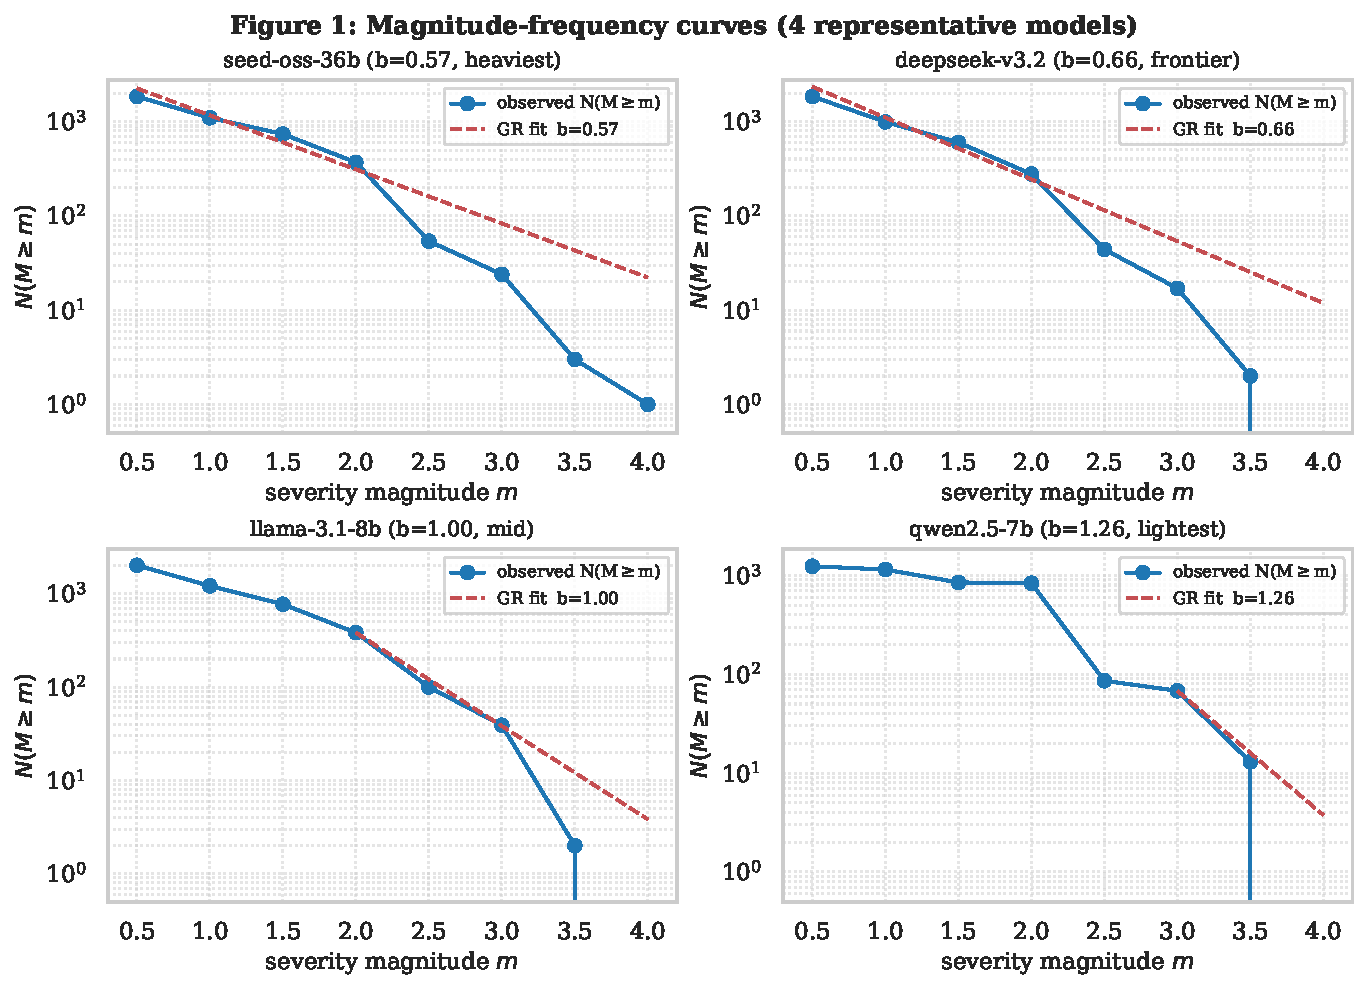
\includegraphics[width=0.8\linewidth]{fig1_flagship.pdf}
\caption{Magnitude-frequency curves for four representative models
spanning the \sdi{} range (heaviest to lightest tail). Dashed red:
Gutenberg--Richter fit. All $21$ models and the $\Delta$BIC heatmap
are in Appendix~\ref{app:supp}.}\label{fig:fig1}
\end{figure}

\subsection{$b$-value as discriminator (Exp.\ 2)}\label{sec:exp2}
Across $\binom{21}{2} = 210$ model pairs, $42$ have $|\Delta\varepsilon|
< 0.05$ and $|\Delta b| > 0.15$. Of those, \textbf{30 have disjoint
95\% CIs on $b$} --- the pre-registered criterion ($\geq 3$) is met by
an order of magnitude. Concretely, \textsc{deepseek-v3.2}
($\varepsilon = 0.586,\, b = 0.655$) and \textsc{ministral-14b}
($\varepsilon = 0.586,\, b = 1.122$) have identical accuracy but a
$b$-value gap of $0.467$ with non-overlapping CIs. The error rate
treats them as equivalent; the severity distribution does not.
\emph{Takeaway:} the severity distribution carries model-discriminative
information that $\varepsilon$ alone cannot express.

\subsection{Negative scaling correlation in dense models
(Exp.\ 5, headline)}\label{sec:exp5}

\paragraph{Result.} Across the 14 dense instruction-tuned models in
our catalog, the Spearman correlation between $\log_{10}$(active
parameters) and the Gutenberg--Richter $b$-value is
\[
  \boxed{\rho_s = -0.689,\qquad p = 0.006,\qquad n_{\text{dense}} = 14.}
\]
Pooling all 21 models (including 7 MoE) gives
$\rho_s = -0.585$ ($p = 0.005$); restricted to MoEs alone, $n = 7$ is
underpowered but the sign is the same ($\rho_s = -0.595$, $p = 0.16$).
Pre-registration called for no clean correlation; the data refute the
null and the direction is opposite the ``bigger models are safer''
intuition. \Cref{fig:fig6} plots the relationship.

\begin{figure}[t]
\centering
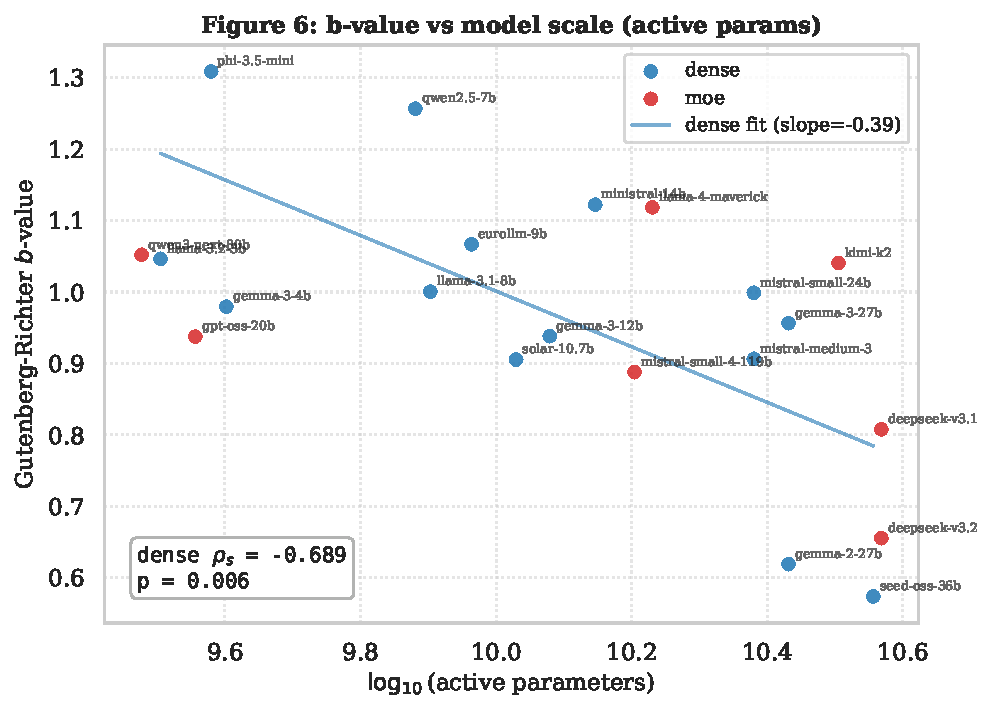
\includegraphics[width=0.7\linewidth]{fig6_scale.pdf}
\caption{\textbf{Headline.} \sdi{} vs.\ active parameter count.
Dense (blue) shows a monotone downward trend; MoE (red) follows the
same sign but is underpowered. Linear fit on the dense subset overlaid.}
\label{fig:fig6}
\end{figure}

\paragraph{Concrete instances.} The two heaviest tails in the catalog
belong to the largest \emph{dense} models we evaluate:
\textsc{seed-oss-36b} ($b = 0.574$, 36B active params) and
\textsc{gemma-2-27b} ($b = 0.619$, 27B). The two lightest tails are
the \emph{smallest} models: \textsc{phi-3.5-mini} ($b = 1.309$, 3.8B)
and \textsc{qwen2.5-7b} ($b = 1.257$, 7.6B). The error rate moves in
the conventional direction over this range --- the largest dense
models are more accurate than the smallest --- yet the severity
distribution of the errors that remain moves the opposite way.

\paragraph{Interpretation.} Larger dense models commit \emph{fewer}
mistakes but the ones they commit are \emph{more severe}. We interpret
this as evidence that capability scaling shifts the residual error
population: small models fail on simple pattern-matching and produce
many low-severity slips; large models fail when they are asked to
integrate many facts confidently and are more likely to produce
coherent, high-severity fabrications. Safety tuning on instruction
data reduces the \emph{frequency} of error but does not necessarily
reduce the \emph{severity} of the residual.

\paragraph{Leave-one-out robustness.} The headline correlation
survives every single-model deletion. Dropping each of the $14$
dense models in turn and recomputing on the remaining $13$, the
Spearman correlation stays negative and significant in
\textbf{$14/14$} drops; the range of LOO $\rho$ is
$[-0.777, -0.612]$ and the worst-case $p$-value is
$0.0263$ (achieved when \textsc{seed-oss-36b}, the largest dense
model, is removed). The finding is not driven by any single point.
Per-drop values appear in Appendix~\ref{app:loo}.

\paragraph{Caveats.} (i) Active parameters are used to normalise MoEs
against dense models, but the MoE subset ($n=7$) is too small to fit
a separate trend that reaches $p<0.05$. (i$'$) The headline correlation
is computed under the model-specific KS-selector for $m_{\min}$,
which targets the upper tail. Under fixed $m_{\min}$ strategies the
correlation flips sign (S5, \S\ref{sec:sensitivity}); the headline
claim is therefore explicitly about the upper-tail slope, not the
bulk decay rate. (i$''$) We estimate \sdi{} from a Gutenberg--Richter
exponential tail for all models regardless of best-fit family; if the
family-native shape parameter (stretching exponent for stretched
exponential, tail exponent for truncated power law, scale for
lognormal) were used as the summary statistic instead, the ranking
could shift for models where the exponential is a poor local
approximation. We leave family-native estimation as a robustness
check in a follow-up release. (ii)
\textsc{llama-3.1-405b-instruct} was excluded from the study (API
rate limits; see \S\ref{sec:limitations}); the largest dense model we
evaluate is $36$B. The trend covers a $\sim 10\times$ range in
active-parameter count, not the full frontier, and should not be
extrapolated into the unobserved $100$B+ dense regime without direct
measurement. (iii) The correlation is computed on model-aggregated
\sdi{} values; Exp.\ 4 (\S\ref{sec:exp4}) shows that domain-level
\sdi{} is model-idiosyncratic, so the headline is about
\emph{whole-model} tail shape, not any particular domain.

\paragraph{Headline robustness suite.}
The dense correlation survives bootstrap ($95\%$ CI $[-0.92, -0.26]$),
exact permutation ($p = 0.0077$ two-sided), Bayesian linear
regression ($\beta = -0.39$, $95\%$ CI $[-0.64,\,-0.14]$,
$P(\beta<0|\text{data}) = 0.999$), and per-tier decomposition (sign
preserved in $4/5$ tiers; T2 individually significant at $p = 0.04$,
Appendix~\ref{app:per_tier}). At $n = 14$ the study is
\emph{borderline} powered (min detectable $|\rho| = 0.701$ at
$\alpha = 0.05$, power $= 0.80$, observed $|\rho| = 0.689$);
split-half $\sdi$ reliability is mean Spearman $0.882$ across
$100$ trials. Full output: \texttt{results/analysis/headline\_robustness.json}.

\paragraph{Accuracy mediates a substantial part of the headline.}
A formal independence test changes the framing. On the $14$-dense
subset, $\sdi$ and $\varepsilon$ are \emph{negatively correlated}
($\rho_s = -0.73$, $p = 0.003$), and $\varepsilon$ itself
\emph{positively} correlates with size
($\rho_s(\log_{10}\text{params},\varepsilon) = +0.59$, $p = 0.026$):
the smallest dense models in our catalog (\textsc{phi-3.5-mini},
\textsc{qwen2.5-7b}) are heavily benchmarked with low $\varepsilon
\approx 0.30$, while larger dense models are more general-purpose
($\varepsilon \approx 0.55$--$0.67$). Partialing $\varepsilon$ out of
$(\log_{10}\text{params}, \sdi)$ via OLS residuals leaves
$\rho_s = -0.29$ ($p = 0.31$, $n=14$) --- sign preserved but no
longer individually significant. Accuracy-stratified halves both
preserve the negative sign ($\rho_s = -0.50$ high-acc, $-0.29$
low-acc; $n=7$ each). \textbf{Revised framing:} $\varepsilon$ and
$\sdi$ are correlated, not independent, in this sample. The
$30/210$ disjoint-CI pairs at matched accuracy (\S\ref{sec:exp2})
still establish that $\sdi$ carries information \emph{beyond}
$\varepsilon$, but our earlier ``independent axes'' language was
too strong; \emph{$\sdi$ is most informative as a discriminator
when comparing models at matched accuracy.}

\paragraph{Verbosity confound.}\label{par:verbosity}
A plausible alternative explanation is that larger dense models
produce longer responses, which expose more surface area for judge
overcalling. We falsify this. On the $13$ dense models with recorded
raw responses, mean response length is \emph{not} correlated with
parameter count ($\rho_s(\log_{10}\text{params},\log_{10}\text{words})
= -0.080$, $p = 0.80$); compare \textsc{gemma-2-27b} (27B, mean
$16.4$ words, third-shortest) with \textsc{ministral-14b} (14B,
$72.6$ words, longest). Length does correlate with overcall rate
($\rho_s = +0.50$, $p = 0.05$), so verbose responses \emph{are}
overcalled more --- but because length is size-orthogonal, this
routes overcall noise away from the size axis. OLS regression of
$\sdi$ on $\log_{10}(\text{params})$ controlling for
$\log_{10}(\text{mean words})$ on the $n=13$ dense subset gives
$\beta_{\text{params}} = -0.38$ (SE $0.13$, $p = 0.013$); the
headline survives the partial-regression test at $p < 0.05$. Full
output: \texttt{results/analysis/verbosity\_check.json}.

\subsection{Predicting catastrophes from micro-errors
(Exp.\ 3)}\label{sec:exp3}
\textbf{Pre-registered hypothesis:} fitting $b$ on tier-1/2 errors
predicts catastrophic-error counts ($M \geq 3.0$) on tiers 4/5 via
Gutenberg--Richter extrapolation. Across 21 models the Spearman
correlation between predicted and observed counts is
\[
  \rho_s = 0.443,\quad p = 0.044,\quad \text{Kendall}~\tau = 0.325.
\]
At a relaxed threshold $M \geq 2.5$, $\rho_s = 0.637$
($p = 0.002$). The result lands in the WEAK band of the pre-registered
schedule (\Cref{fig:fig4}): rank prediction is statistically significant
but \textbf{absolute-rate prediction fails} --- only $4/21$ ($M\geq 3$)
and $1/21$ ($M\geq 2.5$) of models land within $1.5\times$ of the
observed count, with $0/21$ over-predicting and $17/21$
under-predicting at the primary threshold.

\paragraph{Mechanistic explanation.} Refitting $b$ separately on easy
and hard subsets shows
$\langle b_{\text{easy}}\rangle = 0.921$ and
$\langle b_{\text{hard}}\rangle = 0.962$ ($\Delta = -0.041$, std
$0.216$). There is no systematic slope divergence; the under-prediction
is a \emph{level shift}, not a slope mismatch. Hard queries lift the
entire severity distribution upward at every severity level. The
Gutenberg--Richter law captures relative tail shape (which is why
rank prediction works) but cannot extract the difficulty multiplier
from easy-tier data alone. This partial-signal finding is consistent
with Exp.\ 5: $b$ is a \emph{model-level} summary statistic that
carries cross-model discriminative information, but it is not a
cross-regime extrapolator.

% Fig 4 (prediction calibration) relocated to appendix A to save main-text pages.

\subsection{Domain variation (Exp.\ 4)}\label{sec:exp4}
A Friedman test rejects equal $b$-value across the 8 domains
($\chi^2 = 15.94$, $p = 0.026$, $n = 21$). However, Kendall's
coefficient of concordance is \textbf{$W = 0.108$}, meaning that models
\emph{disagree} on which domains have heavy tails. BIO (mean $b$ =
$0.849$) and FIN ($0.841$) are the heaviest-tailed domains on average;
LAW ($1.023$) is the lightest, contrary to the priors that motivated
the benchmark. Domain effects exist but are model-idiosyncratic
(heatmap in Appendix~\ref{app:supp}). This is why the headline
negative-scaling result in \S\ref{sec:exp5} is computed on
model-aggregated \sdi{} values rather than per-domain slopes:
there is no stable domain ranking to average across.


\subsection{Training-pipeline pairs and sensitivity
summary}\label{sec:sensitivity}

Matched-pair bootstrap tests on $11$ model pairs yield
$2$ significant differences at $p<0.05$
(\textsc{llama-3.2-3b vs.\ llama-3.1-8b}, $\Delta\sdi = -0.53$,
$p<0.001$; and \textsc{qwen2.5-7b vs.\ llama-3.1-8b},
$\Delta\sdi = -0.32$, $p = 0.021$); the DeepSeek v3.1 $\to$ v3.2
version bump is \emph{not} significant ($p = 0.87$). The full pair
table is Appendix~\ref{app:pairs}, and within-generation and
version-bump comparisons appear in \Cref{fig:fig7,fig:fig8}
(Appendix~\ref{app:sensitivity}).

Three pre-registered sensitivity checks were executed. \textbf{S1
(scale coarsening)} \emph{fails}: collapsing the $9$-point scale to
a $7$-point grid gives $\rho_s = 0.43$, and to $5$ levels gives
$\rho_s = 0.16$, both well below the $0.85$ stability threshold ---
the $9$-point grid is load-bearing. \textbf{S2 (overcall correction)}
\emph{narrowly fails} at $\rho_s = 0.847$, $0.003$ below the
threshold; the \sdi{} ranking is robust to within the margin but
not strictly above it. \textbf{S3 (subsample stability)}
\emph{passes}: median coefficient of variation on \sdi{} under
$50\%$ subsampling is $0.143$. Full S1--S3 figures are
Appendix~\ref{app:sensitivity}.

\paragraph{S5: $m_{\min}$ sensitivity.} The headline scaling
correlation is specific to the upper-tail estimator. Under our
default model-specific KS-selector $\rho_s = -0.689$ ($p = 0.006$);
under fixed $m_{\min} = 1.5$ $\rho_s = +0.837$ ($p = 0.0002$); under
Clauset-style $\geq 100$ exceedances (which selects $m_{\min} = 0.5$
for every model) $\rho_s = +0.793$ ($p = 0.0007$). \emph{The sign
flips.} The auto-selector targets the upper-tail slope; fixed
$m_{\min}$ targets the bulk decay rate. Both are real --- larger
dense models commit fewer small slips (steeper bulk) and a relatively
higher fraction of catastrophic fabrications (shallower upper tail).
\textbf{The paper's headline applies to the upper-tail slope only;
the bulk slope moves the opposite way.} Full table:
Appendix~\ref{app:s5}.

\paragraph{Deployment implications.}\label{sec:deployment}
\Cref{fig:fig10} (Appendix~\ref{app:deployment}) translates the
empirical severity distributions into expected catastrophic
($M \geq 3.0$) and severe ($M \geq 2.5$) events per million queries
under i.i.d.\ deployment. Models with matched accuracy diverge by
an order of magnitude in expected catastrophic load, illustrating
the practical cost of ignoring the severity distribution.

% =====================================================================
\section{Discussion}\label{sec:discussion}

\paragraph{Three layers in decreasing order of surprise.}
Our findings sit on three layers. \emph{Layer 1 --- severity
distributions exist and discriminate models} (Exp.\ 1--2): this is
foundational but unsurprising to anyone who has seen LLM failure
modes up close. \emph{Layer 2 --- the negative scaling correlation}
(Exp.\ 5): among dense instruction-tuned open-weight models, the
\sdi{} anti-correlates with $\log_{10}$(active params) at
$\rho_s = -0.689$. Larger dense models are more accurate but their
residual errors are more severe. This is the finding we did not
expect, it survives leave-one-out deletion ($14/14$ drops preserve
both sign and significance), and it is the claim with the most
immediate evaluation-practice impact: two vendors advertising the
same benchmark accuracy can have an order-of-magnitude gap in
catastrophic event rate, and the direction of that gap favours the
smaller model. \emph{Layer 3 --- partial prediction} (Exp.\ 3):
micro-error measurements rank-order catastrophic counts with
moderate signal but do not produce calibrated absolute-rate
predictions.

\paragraph{Future work: tighter fits enable tail extrapolation.}
We conjecture that Layer 3's failure is a data-quantity problem,
not a structural one. With $\sim 800$ errors per model, the tail
above $M \geq 3$ contains only $10$--$50$ events, and bootstrap
CIs on \sdi{} are too wide to support cross-regime extrapolation.
A $10\times$ expansion of the benchmark would tighten the fits
enough to test two follow-ups: (i) whether the difficulty
multiplier is regressible from easy-tier data directly, converting
the rank signal into a calibrated extrapolator; and (ii) whether
the Layer 2 scaling relation can be localised to a specific
exceedance probability $\Pr(M \geq m^*)$ at an operationally
meaningful threshold.

\paragraph{Distributional mechanism (speculative).} The dominance
of stretched-exponential and lognormal best-fits over pure power
laws is consistent with a \emph{multiplicative} noise model of
error severity --- failure severity as a product of stage-level
errors (retrieval, reasoning, generation) rather than a sum. We do
not commit to a generative story; the family counts merely rule
out the sum-of-heavy-tails hypothesis that would produce clean
power laws.

\section{Limitations and misuse}\label{sec:limitations}

\paragraph{Judge overcalling and scale resolution.} A $340$-item
manual audit classifies $33.5\%$ of judge score-$2.0$ verdicts as
overcalls; verbose responses are overcalled more (Appendix~\ref{app:overcall}).
The headline survives bootstrap overcall correction
($\rho_s = 0.847$, S2, just below the $0.85$ threshold) and the
verbosity covariate (\S\ref{par:verbosity}). Sensitivity S1 also
shows that collapsing the $9$-point severity grid to $7$ points or
$5$ levels destroys the \sdi{} ranking ($\rho_s = 0.43$ and
$0.16$); practitioners must use the full grid.

\paragraph{Model coverage and scope.} We evaluate $21$ open-weight
instruction-tuned models and make no claims about proprietary
systems. Frontier-dense coverage is constrained:
\textsc{llama-3.1-405b-instruct}, \textsc{gpt-oss-120b}, and
\textsc{minimax-m2.5} were excluded from the main analysis after
rate-limit exhaustion. We re-attempted \textsc{llama-3.1-405b}
during revision; one-shot calls succeed on a single key, but at
the $32$-way concurrency required for a $4{,}000$-query cohort
evaluation, $87.5\%$ of requests return $429$ or $403$
($403/3314$ valid responses, $12.2\%$ success). This is too sparse
for a stable upper-tail $\sdi$ fit and we exclude $405$B from the
main analysis. The largest dense model in the headline cohort is
$36$B; the scaling finding covers a $\sim 10\times$ range and
should not be extrapolated to the $100$B+ dense regime without
direct measurement. Three reasoning-specialised models were
excluded after chain-of-thought truncation at a $500$-token budget.
Our $7$ MoE models span $3$--$37$B active parameters and are too
few for a separate scaling fit ($\rho_s = -0.595$, $p = 0.159$,
$n=7$ --- same sign, not significant).

\paragraph{Human validation, prediction, and misuse.} The
$340$-item human-scored subset was rated by a single expert rater;
inter-rater ICC was not formally computed. Experiment 3 fails its
primary pre-registered criterion ($\rho_s \geq 0.75$ at $M \geq
3$); only the moderate rank signal $\rho_s = 0.443$ ($p = 0.044$)
holds. Because the $9$-level scale, the scoring pipeline and the
benchmark queries are released openly, optimising-against-the-test
is detectable: an adversarial fine-tune will not reproduce the
public pipeline's outputs on unreleased held-out queries. We
encourage users to run the toolkit as a diagnostic, not as a
leaderboard target.

% =====================================================================
\section{Conclusion}\label{sec:conclusion}

Larger dense open-weight LLMs concentrate their remaining errors in
the upper tail ($\rho_s(\log_{10}\text{params},\, \sdi) = -0.689$,
$p = 0.006$, $n_{\text{dense}} = 14$, $14/14$ LOO). The sign is
specific to the upper-tail estimator; under fixed $m_{\min}$ the
sign flips, indicating that larger dense models commit fewer small
slips and a relatively higher fraction of catastrophic ones. The
\sdi{} discriminates $30/210$ model pairs at matched accuracy ---
direct evidence that it carries information beyond $\varepsilon$
even though $\varepsilon$ and $\sdi$ are themselves correlated
($\rho_s = -0.73$). The headline recommendation is methodological:
\emph{report \sdi{} alongside $\varepsilon$ --- they carry
overlapping but distinguishable information, and the discriminative
gap is large enough to matter at matched accuracy.}

% ---------------------------------------------------------------------
\bibliographystyle{plainnat}
\bibliography{references}

\appendix

% =====================================================================
\section{Supplementary figures (Exp.\ 1, 3, and 4)}\label{app:supp}

\Cref{fig:fig4} is the prediction calibration plot for
Experiment~3 (two panels: the pre-registered $M \geq 3.0$
threshold and the exploratory $M \geq 2.5$ threshold).
\Cref{fig:fig2} gives the full $21$-model magnitude-frequency grid
(small multiples) that \Cref{fig:fig1} summarises with four
representative models. \Cref{fig:fig3} is the BIC heatmap showing
$\Delta$BIC between each candidate distribution family and the
BIC-best for each model (stars mark the selected family).
\Cref{fig:fig5} is the $21 \times 8$ model-by-domain \sdi{}
heatmap.

\begin{figure}[h]
\centering
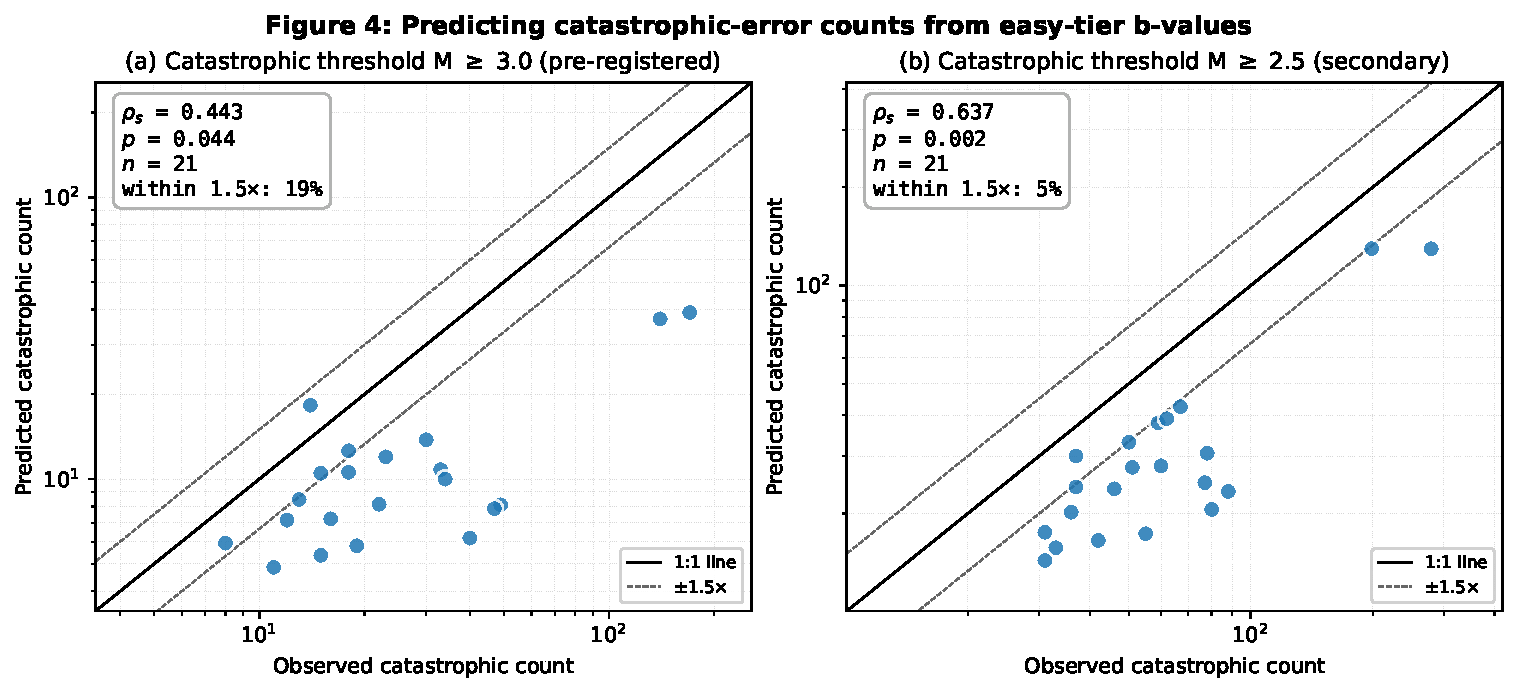
\includegraphics[width=0.85\linewidth]{fig4_prediction_calibration.pdf}
\caption{Predicted vs.\ observed catastrophic counts per model for
Experiment~3. \textbf{Left:} pre-registered $M \geq 3.0$ threshold,
$\rho_s = 0.443$. \textbf{Right:} exploratory $M \geq 2.5$
threshold, $\rho_s = 0.637$. Solid line is identity, dashed lines
mark $\pm 1.5\times$. Only $4/21$ models land within $1.5\times$ at
$M \geq 3.0$; $0/21$ over-predict.}\label{fig:fig4}
\end{figure}

\begin{figure}[h]
\centering
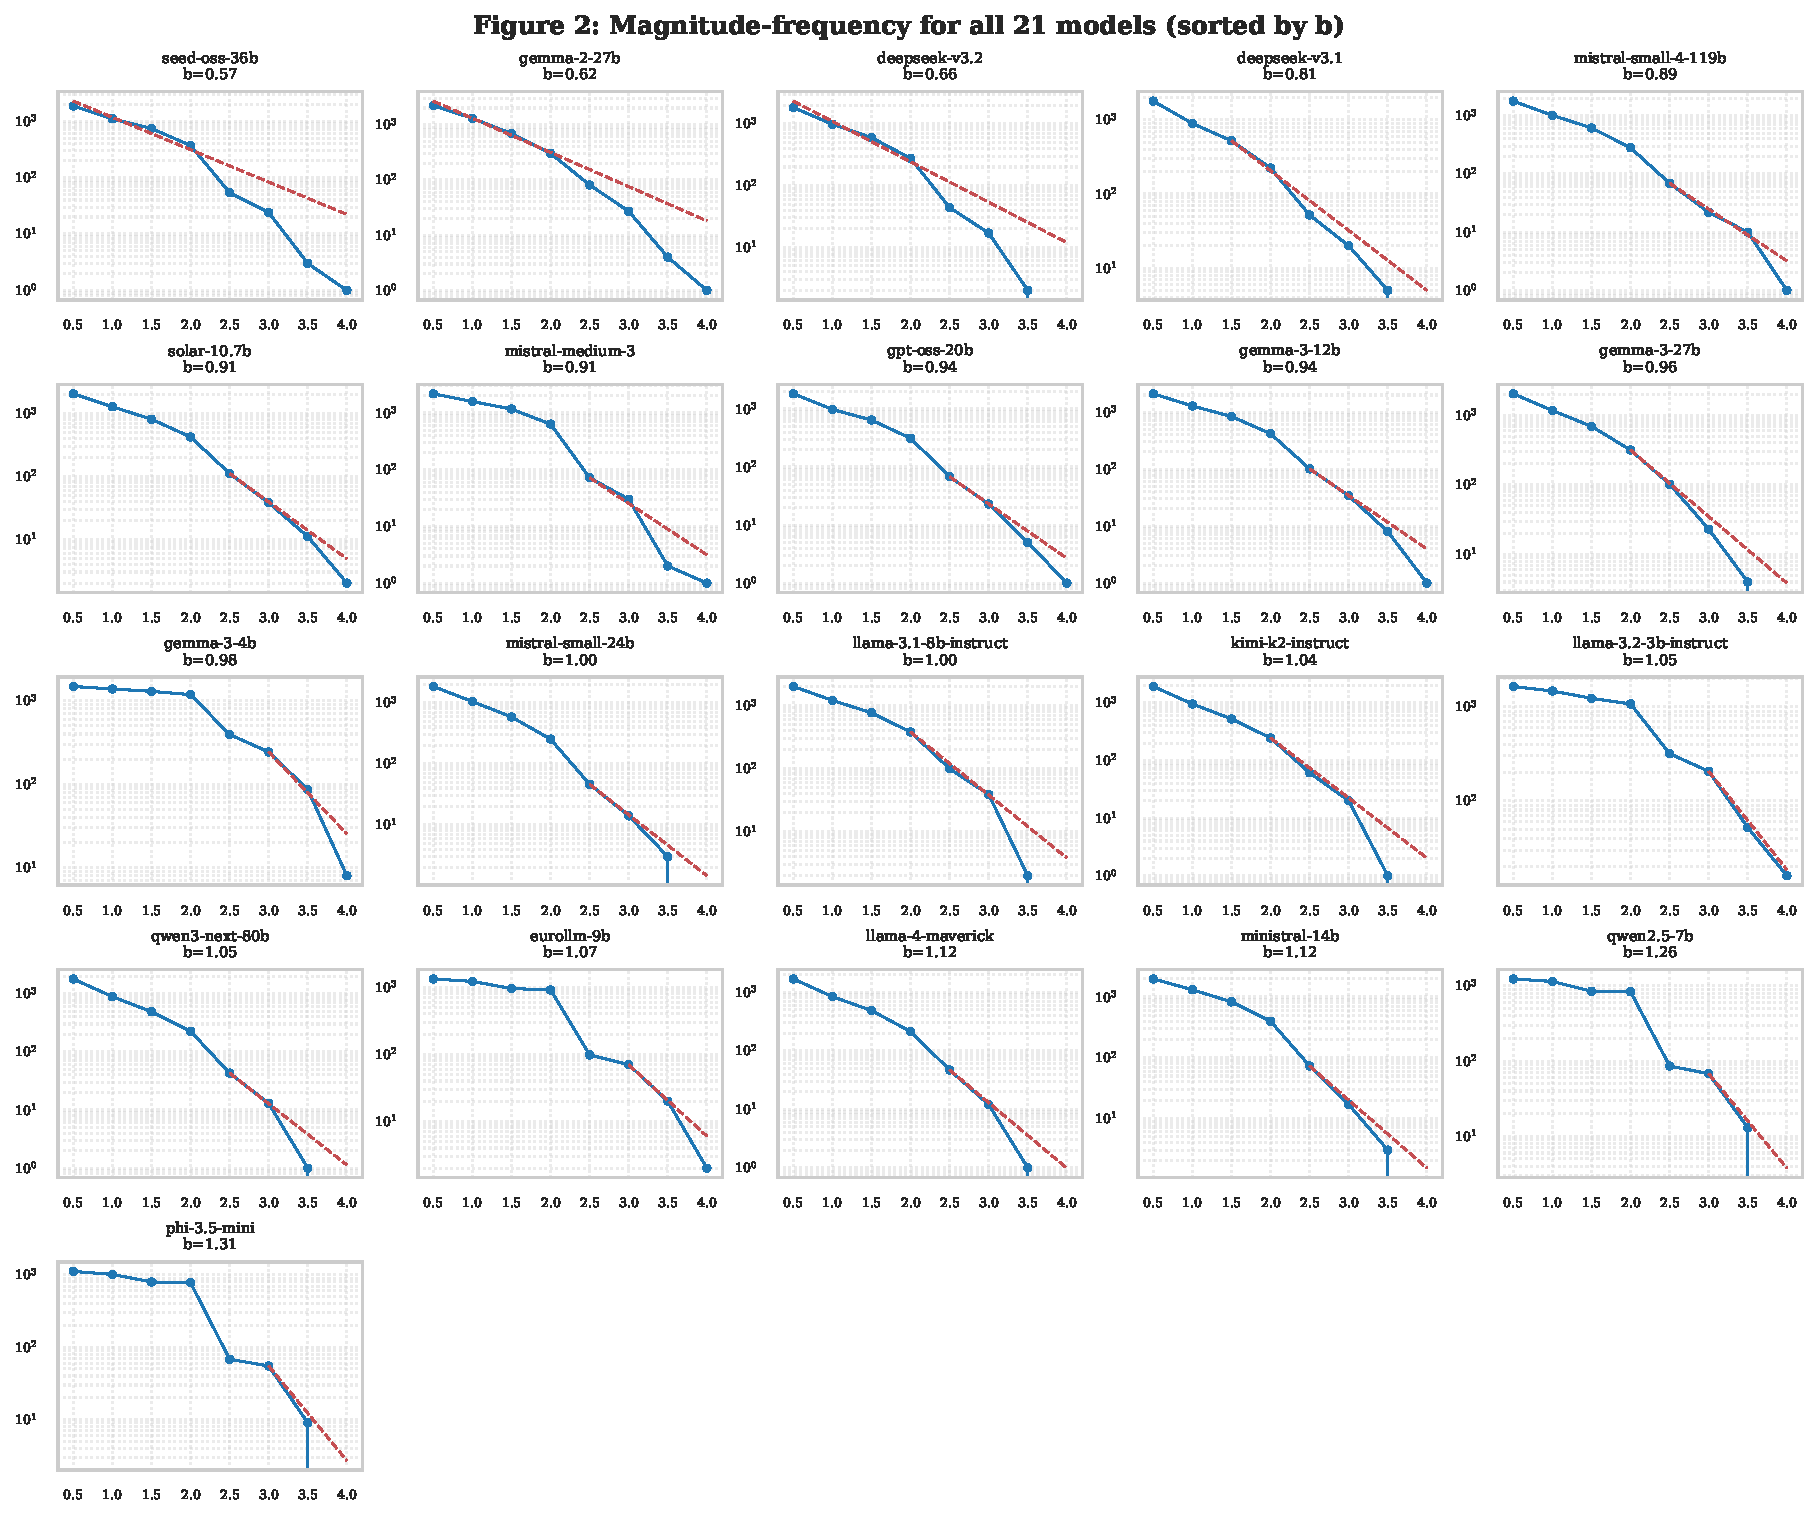
\includegraphics[width=0.95\linewidth]{fig2_grid.pdf}
\caption{All $21$ models sorted by \sdi{} (heaviest-tailed at top).
Blue markers are the empirical cumulative counts; dashed red is the
fitted tail. Compact form of \Cref{fig:fig1}.}\label{fig:fig2}
\end{figure}

\begin{figure}[h]
\centering
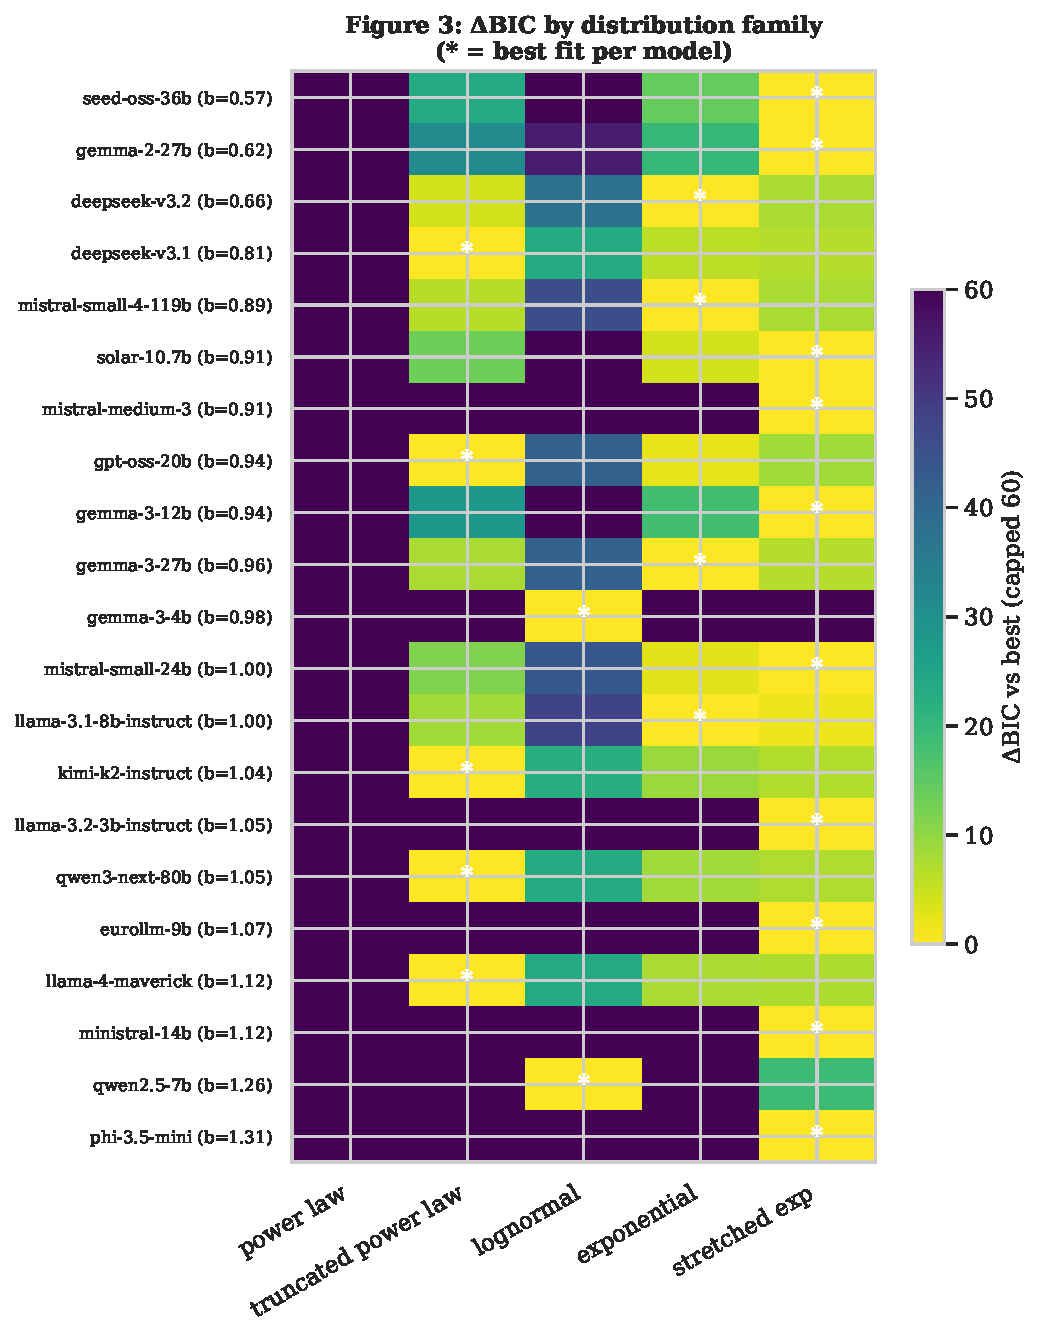
\includegraphics[width=0.55\linewidth]{fig3_bic_heatmap.pdf}
\caption{$\Delta$BIC between each distribution family and the
best-fit family for each of the $21$ models, capped at $60$. Stars
mark the selected family.}\label{fig:fig3}
\end{figure}

\begin{figure}[h]
\centering
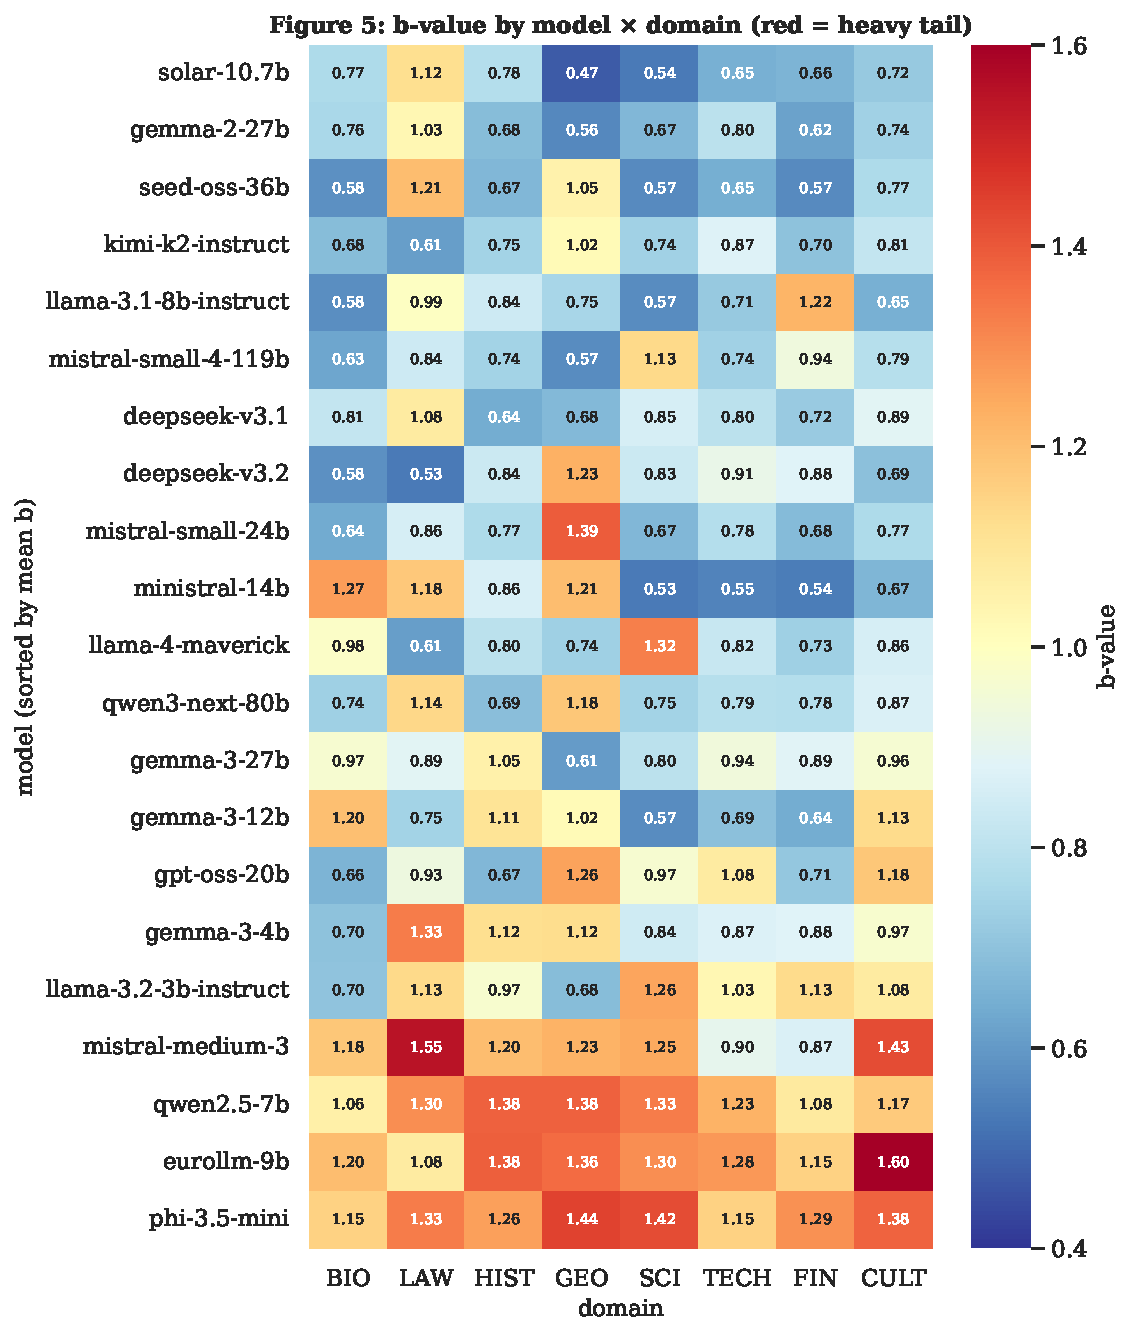
\includegraphics[width=0.85\linewidth]{fig5_domain_heatmap.pdf}
\caption{\sdi{} by model $\times$ domain. Red = heavier tail. Per-model
rows are sorted by mean \sdi{}. Kendall $W = 0.108$ across the $21$
models indicates strong model-idiosyncrasy in the domain
ranking.}\label{fig:fig5}
\end{figure}

% =====================================================================
\section{Full 21-model results table}\label{app:models}

\Cref{tab:full21} reports each model's \sdi{} with $95\%$ bootstrap
confidence interval, the selected $m_{\min}$, the number of events
at or above $m_{\min}$, the total error count, the error rate, and
the BIC-best distribution family. Rows are sorted by \sdi{}
(heaviest tail first). Active-parameter counts and architecture
labels (dense vs MoE) appear in Appendix~\ref{app:loo}.

\begin{table}[h]
\centering
\small
\begin{tabular}{l r r l r r r l}
\toprule
model & \sdi{} & $95\%$ CI & $m_{\min}$ & $n_{\geq m_{\min}}$ & $n_{\text{err}}$ & $\varepsilon$ & best fit \\
\midrule
\textsc{seed-oss-36b}            & 0.574 & [0.555, 0.593] & 0.5 & 2260 & 2260 & 0.568 & stretched exp \\
\textsc{gemma-2-27b}             & 0.619 & [0.600, 0.639] & 0.5 & 2665 & 2665 & 0.666 & stretched exp \\
\textsc{deepseek-v3.2}           & 0.655 & [0.632, 0.679] & 0.5 & 2340 & 2340 & 0.587 & exponential \\
\textsc{deepseek-v3.1}           & 0.808 & [0.758, 0.863] & 1.5 &  523 & 2278 & 0.571 & trunc.\ power law \\
\textsc{mistral-small-4-119b}    & 0.888 & [0.744, 1.080] & 2.5 &   69 & 2311 & 0.579 & exponential \\
\textsc{solar-10.7b}             & 0.905 & [0.794, 1.042] & 2.5 &  111 & 2571 & 0.644 & stretched exp \\
\textsc{mistral-medium-3}        & 0.906 & [0.792, 1.042] & 2.5 &   72 & 2334 & 0.589 & stretched exp \\
\textsc{gpt-oss-20b}             & 0.938 & [0.798, 1.114] & 2.5 &   68 & 2341 & 0.586 & trunc.\ power law \\
\textsc{gemma-3-12b}             & 0.938 & [0.824, 1.076] & 2.5 &  101 & 2521 & 0.631 & stretched exp \\
\textsc{gemma-3-27b}             & 0.956 & [0.885, 1.040] & 2.0 &  316 & 2500 & 0.630 & exponential \\
\textsc{gemma-3-4b}              & 0.979 & [0.908, 1.063] & 3.0 &  243 & 1497 & 0.387 & lognormal \\
\textsc{mistral-small-24b}       & 0.999 & [0.832, 1.211] & 2.5 &   46 & 2265 & 0.566 & stretched exp \\
\textsc{llama-3.1-8b}            & 1.001 & [0.923, 1.082] & 2.0 &  383 & 2429 & 0.607 & exponential \\
\textsc{kimi-k2}                 & 1.041 & [0.948, 1.147] & 2.0 &  245 & 2460 & 0.615 & trunc.\ power law \\
\textsc{llama-3.2-3b}            & 1.046 & [0.942, 1.169] & 3.0 &  206 & 1750 & 0.450 & stretched exp \\
\textsc{qwen3-next-80b}          & 1.052 & [0.879, 1.266] & 2.5 &   43 & 2365 & 0.592 & trunc.\ power law \\
\textsc{eurollm-9b}              & 1.067 & [0.935, 1.241] & 3.0 &   70 & 1356 & 0.344 & stretched exp \\
\textsc{llama-4-maverick}        & 1.118 & [0.938, 1.338] & 2.5 &   47 & 2205 & 0.553 & trunc.\ power law \\
\textsc{ministral-14b}           & 1.122 & [0.968, 1.307] & 2.5 &   73 & 2340 & 0.586 & stretched exp \\
\textsc{qwen2.5-7b}              & 1.257 & [1.114, 1.441] & 3.0 &   68 & 1247 & 0.316 & lognormal \\
\textsc{phi-3.5-mini}            & 1.309 & [1.124, 1.517] & 3.0 &   55 & 1126 & 0.285 & stretched exp \\
\bottomrule
\end{tabular}
\caption{Full 21-model \sdi{} table. Bootstrap CIs from $n=2000$
resamples.}\label{tab:full21}
\end{table}

% =====================================================================
\section{Query benchmark construction}\label{app:benchmark}

\textsc{Errorquake-4k} was generated by a dense frontier model
prompted to produce stratified queries in eight domains and five
difficulty tiers, then verified by an independent dual-judge audit
that flagged tier-miscalibrated cells. Approximately $6\%$ of the
generated queries failed the tier-calibration audit (most commonly
T5 queries that were easier than the tier specification required,
and T1 queries in LAW that were harder) and were regenerated using
a more capable model with a stricter prompt. Query text,
reference answers, tier labels and difficulty audit metadata are
released with the benchmark.

% =====================================================================
\section{Scoring and judge prompts}\label{app:prompts}

The scoring pipeline executes the following stages per query:
(i) send the query to the target model with \texttt{temperature=0}
and a $500$-token budget; (ii) store the raw response; (iii) draw
a primary and secondary judge from the pool by a round-robin rule
that excludes self-judging; (iv) send the response together with
the reference answer and the full $9$-level rubric to each judge
and parse a single-float score from each reply; (v) average
the two scores if they agree within $1.0$, else invoke a
tiebreaker judge and take the median. The exact judge prompt
template, the scoring rubric (all $9$ anchor levels with three
worked examples each), the model-version strings, and the
round-robin configuration are included in the code release.

% =====================================================================
\section{Error-severity scale anchors}\label{app:scale}

The $9$-level continuous severity scale has anchors at
$\{0.0, 0.5, 1.0, 1.5, 2.0, 2.5, 3.0, 3.5, 4.0\}$ with the following
semantic labels:

\begin{description}\itemsep 2pt
\item[0.0 --- correct.] The response answers the query accurately
and completely.
\item[0.5 --- trivial imprecision.] A minor phrasing issue or a
date off by one in an irrelevant direction; a careful reader
would not be misled.
\item[1.0 --- minor imprecision.] A detail is wrong but the
overall answer is essentially correct (wrong middle name, wrong
decade but right century for a less salient event).
\item[1.5 --- moderate imprecision with possible misdirection.]
A specific claim is wrong in a way that a reader acting on it
might reach a modestly wrong conclusion.
\item[2.0 --- moderate error.] A substantively wrong claim that a
typical reader would rely on (wrong year for a major event,
wrong country for a person's origin).
\item[2.5 --- substantial error.] Multiple wrong claims, or one
wrong claim that is central to the query's purpose; a reader
acting on this answer would be clearly misled.
\item[3.0 --- major error.] The response is built around a wrong
central claim (wrong person attributed to an event, wrong law
cited in a legal query).
\item[3.5 --- minor fabrication.] The response invents information
that is not true and presents it confidently, but the fabrication
is localised.
\item[4.0 --- major fabrication.] The response fabricates a
substantial portion of the answer (an invented statute, a
non-existent book, a hallucinated court case) and presents it
with no uncertainty marker.
\end{description}

Each level has three worked examples released with the benchmark.
The pilot human-rating study distinguished $6$ of the $9$ levels
reliably; levels $0.5$, $1.5$, $2.5$, $3.5$ were used less often
by the human rater and less often still by the LLM judges
(Appendix~\ref{app:overcall}).

% =====================================================================
\section{Overcall diagnostic (clearest examples)}\label{app:overcall}

We manually classified $340$ score-$2.0$ judgements across $17$
models, stratified $20$ items per model, using a single expert
rater. Each item was placed into one of three categories:
\emph{genuine} (the judge's $2.0$ matches what a human would
assign), \emph{ambiguous} (the rater thought either $0.5$/$1.0$ or
$2.0$ was defensible), or \emph{overcall} (the judge marked $2.0$
for a response that a human would score $0.0$ or $0.5$).

\textbf{Overall:} $163/340$ genuine ($47.9\%$), $63/340$ ambiguous
($18.5\%$), $114/340$ overcall ($33.5\%$). Per-model overcall
rates are reported in \Cref{fig:fig12}. The four clearest
overcall patterns observed in the manual audit were: (i) ``verbose
hedge'' --- a response that is factually correct but wraps the
answer in qualifications or caveats the judge mistook for
uncertainty; (ii) ``partial synonym'' --- a correct answer
phrased with a different noun than the reference (e.g.,
``emperor'' vs ``king'' for a historical ruler who used both
titles); (iii) ``pedantic detail missing'' --- the correct answer
but without a minor qualifying phrase the judge required; and
(iv) ``correct but rounded'' --- a correct answer rounded to a
different precision than the reference.

% =====================================================================
\section{Experiment 3 per-model breakdown}\label{app:exp3}

\Cref{fig:fig4} aggregates the prediction results; the per-model
breakdown (predicted vs observed catastrophic counts at
$M \geq 3.0$ and $M \geq 2.5$, the ratio, and whether each model
lands within $1.5\times$ of the observed) is released as
\texttt{results/analysis/exp3\_prediction.json}. The mechanistic
diagnostic --- refitting the \sdi{} separately on easy and hard
tiers --- is in \texttt{exp3\_diagnostic.json}; mean
$\Delta \sdi_{\text{easy}-\text{hard}} = -0.041$ (std $0.216$),
$10/21$ models have easy steeper and $11/21$ have hard steeper.

% =====================================================================
\section{Leave-one-out scaling robustness}\label{app:loo}

\Cref{tab:loo} gives the per-drop values from the leave-one-out
robustness check on the Exp.~5 headline correlation. Dropping each
of the $14$ dense models in turn and recomputing the Spearman
correlation between $\log_{10}(\text{active params})$ and \sdi{}
on the remaining $13$ models, the correlation stays negative and
significant in all $14$ drops. The worst-case $p$-value
($p = 0.0263$) is achieved when \textsc{seed-oss-36b}, the
heaviest-tailed and largest dense model, is removed.

\begin{table}[h]
\centering
\small
\begin{tabular}{l r r}
\toprule
model dropped & LOO Spearman $\rho$ & $p$-value \\
\midrule
\textsc{ministral-14b}           & $-0.777$ & $0.0018$ \\
\textsc{gemma-3-4b}              & $-0.736$ & $0.0042$ \\
\textsc{solar-10.7b}             & $-0.725$ & $0.0051$ \\
\textsc{gemma-3-12b}             & $-0.711$ & $0.0065$ \\
\textsc{llama-3.2-3b}   & $-0.705$ & $0.0071$ \\
\textsc{mistral-small-24b}       & $-0.704$ & $0.0072$ \\
\textsc{eurollm-9b}              & $-0.700$ & $0.0078$ \\
\textsc{gemma-3-27b}             & $-0.680$ & $0.0106$ \\
\textsc{llama-3.1-8b}   & $-0.678$ & $0.0109$ \\
\textsc{qwen2.5-7b}              & $-0.667$ & $0.0128$ \\
\textsc{mistral-medium-3}        & $-0.663$ & $0.0135$ \\
\textsc{phi-3.5-mini}            & $-0.634$ & $0.0201$ \\
\textsc{gemma-2-27b}             & $-0.622$ & $0.0233$ \\
\textsc{seed-oss-36b}            & $-0.612$ & $0.0263$ \\
\bottomrule
\end{tabular}
\caption{Leave-one-out Spearman correlations on the Exp.~5 headline.
All $14$ drops preserve sign and significance. Baseline
$\rho_s = -0.689$, $p = 0.006$ ($n = 14$).}\label{tab:loo}
\end{table}

% =====================================================================
\section{Training-pipeline pair comparisons}\label{app:pairs}

\Cref{tab:pairs} lists the $11$ matched pairs tested. For each pair
we estimate the \sdi{} on the two models separately, fit at a
shared $m_{\min}$, and report the bootstrap-resampled difference
distribution.

\begin{table}[h]
\centering
\small
\begin{tabular}{l l l r r l}
\toprule
pair & hypothesis & $\Delta\sdi$ & $95\%$ CI & $p$ & verdict \\
\midrule
llama-3.2-3b vs 3.1-8b          & within-Llama scale    & $-0.532$ & $[-0.749,\,-0.287]$ & $0.000$ & sig \\
qwen2.5-7b vs llama-3.1-8b      & family at $8$B        & $-0.317$ & $[-0.556,\,-0.040]$ & $0.021$ & sig \\
gemma-3-12b vs 27b              & within-Gemma-3 scale  & $-0.198$ & $[-0.389,\,+0.008]$ & $0.057$ & marg.\ \\
gemma-3-12b vs ministral-14b    & family at $\sim 13$B  & $-0.189$ & $[-0.408,\,+0.030]$ & $0.091$ & n.s. \\
gemma-3-4b vs 12b               & within-Gemma-3 scale  & $-0.169$ & $[-0.453,\,+0.069]$ & $0.205$ & n.s. \\
mistral-24b vs gemma-3-27b      & family at $\sim 25$B  & $-0.132$ & $[-0.378,\,+0.127]$ & $0.301$ & n.s. \\
mistral-24b vs medium-3         & Mistral tier          & $+0.098$ & $[-0.143,\,+0.366]$ & $0.446$ & n.s. \\
gemma-2-27b vs gemma-3-27b      & generation upgrade    & $+0.040$ & $[-0.076,\,+0.155]$ & $0.496$ & n.s. \\
deepseek-v3.1 vs v3.2           & minor version bump    & $-0.006$ & $[-0.071,\,+0.063]$ & $0.872$ & n.s. \\
llama-4-maverick vs ministral-14b & MoE vs dense $\sim 14$B & $+0.001$ & $[-0.272,\,+0.281]$ & $0.982$ & n.s. \\
gemma-3-4b vs 27b               & scale span            & $+0.023$ & $-$ & $-$ & insuf.\ \\
\bottomrule
\end{tabular}
\caption{Training-pipeline pair tests. $2/11$ pairs reach
$p < 0.05$; notably, the DeepSeek version bump v3.1 $\to$ v3.2 does
\emph{not} significantly change the severity distribution.}\label{tab:pairs}
\end{table}

\begin{figure}[h]
\centering
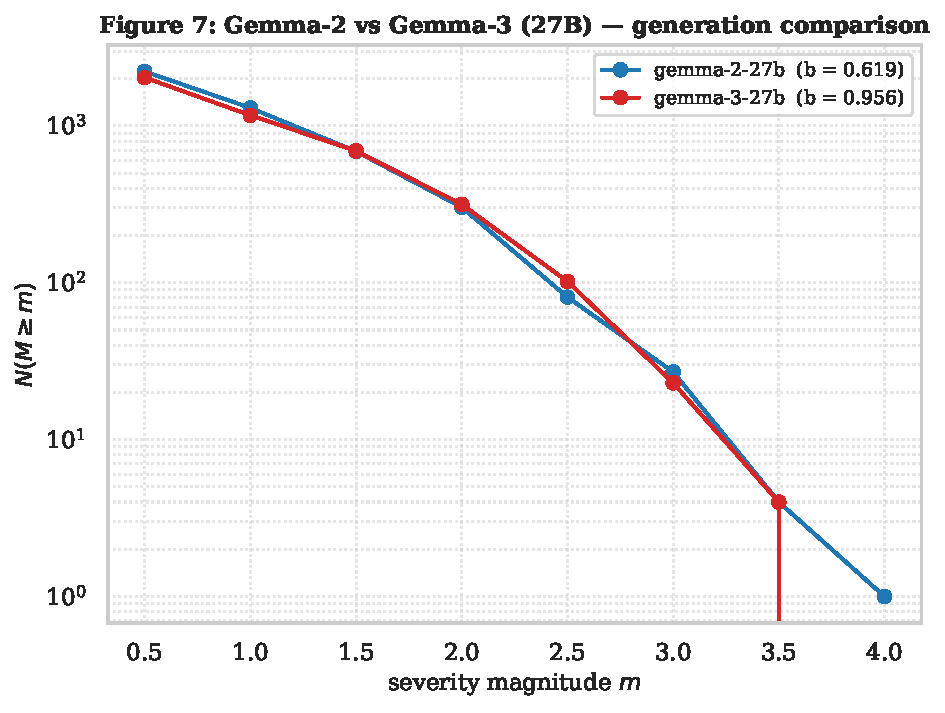
\includegraphics[width=0.65\linewidth]{fig7_gemma_pair.pdf}
\caption{Gemma-2 vs.\ Gemma-3 at 27B (generation upgrade).
Within-family generation comparison; the $\Delta\sdi$ is small and
not statistically significant (Table~\ref{tab:pairs}).}\label{fig:fig7}
\end{figure}

\begin{figure}[h]
\centering
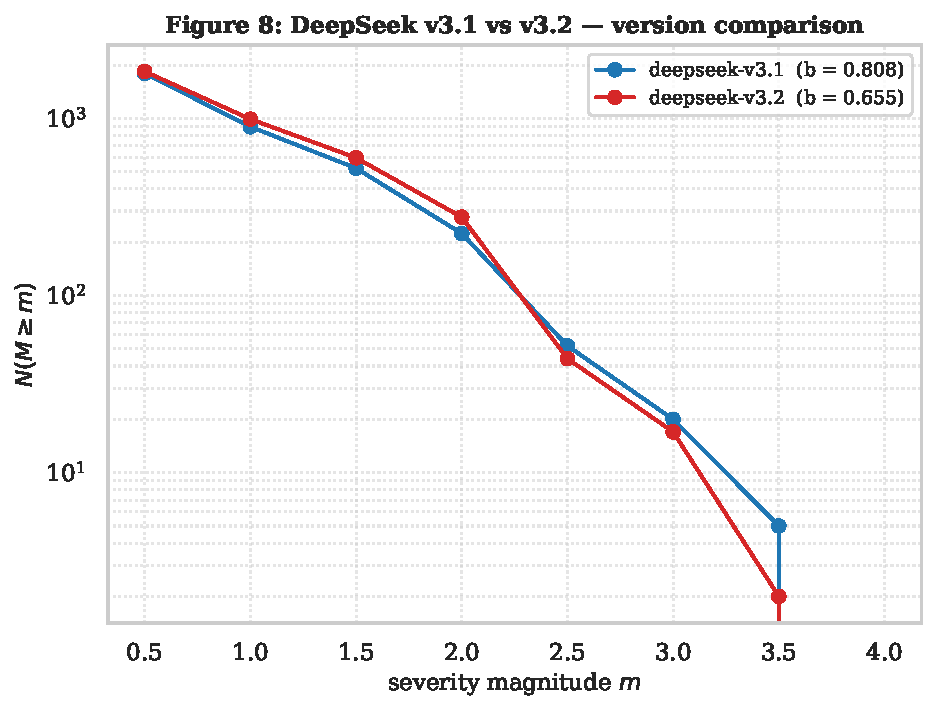
\includegraphics[width=0.65\linewidth]{fig8_deepseek.pdf}
\caption{DeepSeek v3.1 vs.\ v3.2 (minor version bump). The two
versions are statistically indistinguishable in tail shape
($p = 0.872$, Table~\ref{tab:pairs}).}\label{fig:fig8}
\end{figure}

% =====================================================================
\section{Deployment table (full)}\label{app:deployment}

\Cref{fig:fig10} plots expected catastrophic ($M \geq 3.0$) and
severe ($M \geq 2.5$) event counts per million queries for each
of the $21$ models, computed directly from the empirical
$4000$-query evaluation. \textsc{gemma-3-4b} and
\textsc{llama-3.2-3b} have the highest catastrophic rate
(${\sim}10{,}000$ per million), consistent with their small dense
size and correspondingly flat tails at the upper end of the
$9$-point scale. Fitted \sdi{} values provide an alternative
tail-shape summary but are not a calibrated extrapolator
(\S\ref{sec:exp3}).

\begin{figure}[h]
\centering
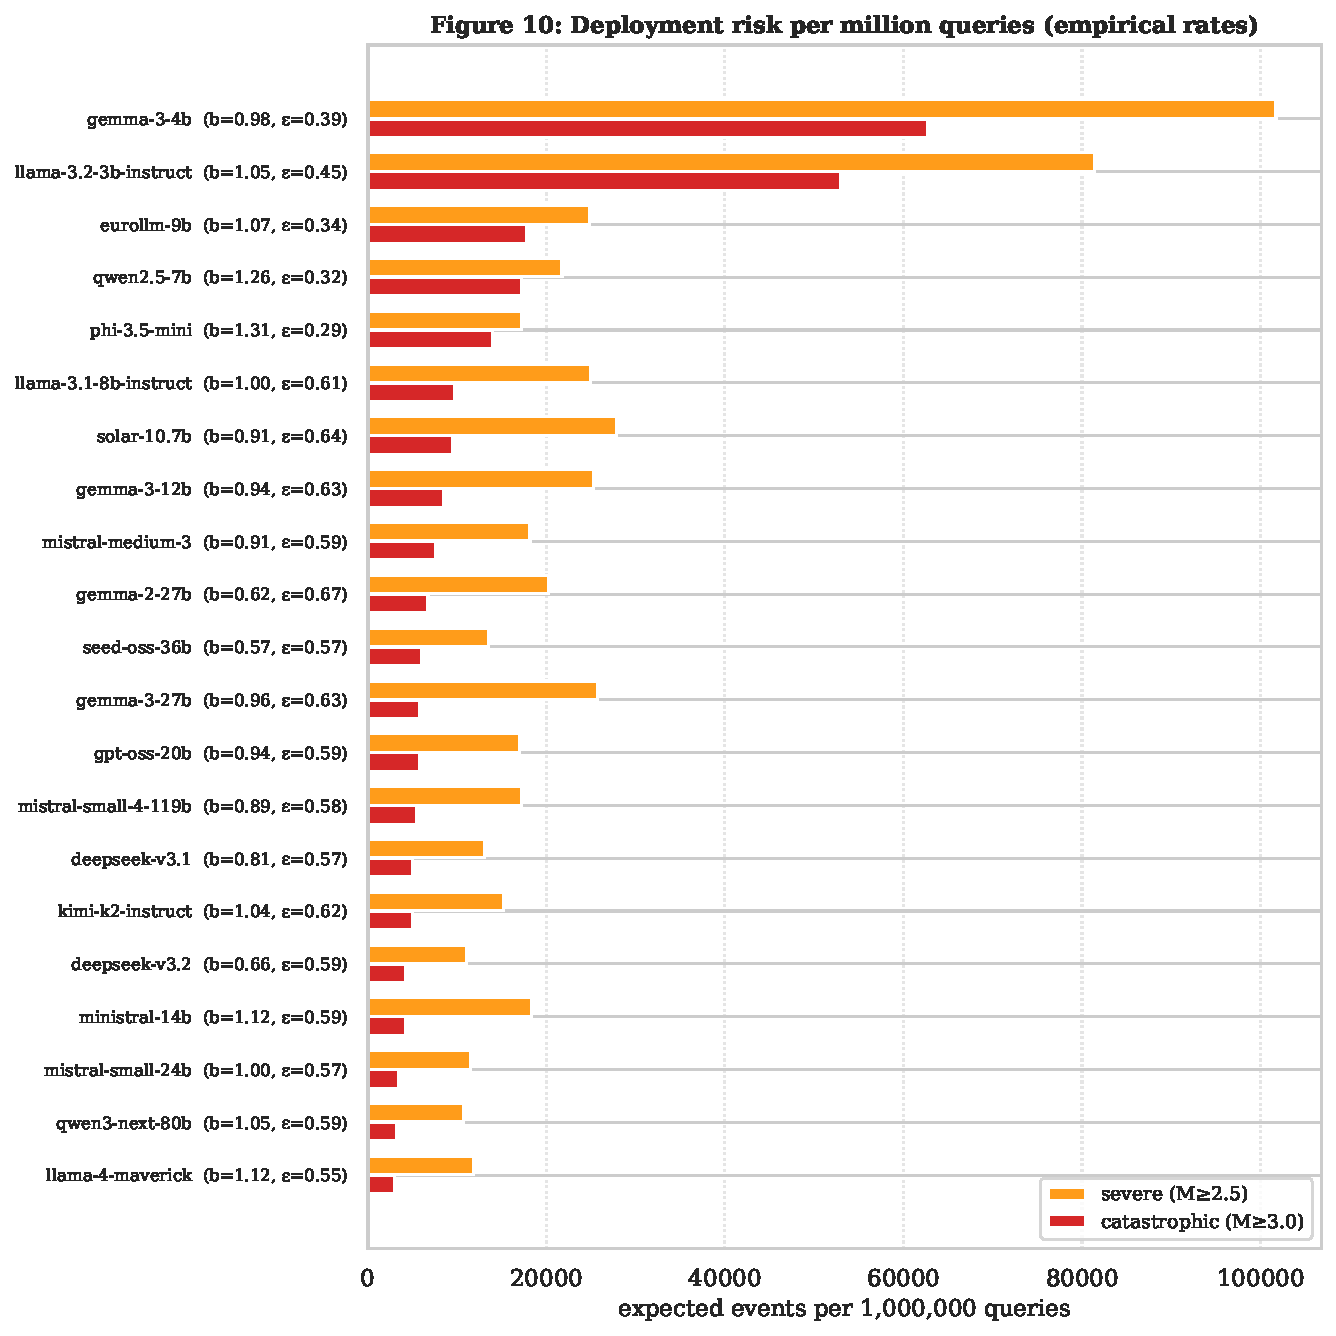
\includegraphics[width=0.85\linewidth]{fig10_deployment.pdf}
\caption{Empirical event rate per million queries for $21$ models,
sorted by catastrophic count ($M \geq 3.0$, red bars) with severe
($M \geq 2.5$, orange bars) for comparison.}\label{fig:fig10}
\end{figure}

% =====================================================================
\section{Inter-judge agreement (per-model)}\label{app:judges}

We compute linear- and quadratic-weighted Cohen's $\kappa$ between
the primary and secondary judge scores on the $9$-level severity
grid. The pooled values across $60{,}568$ dual-scored records are
$\kappa_{\text{lin}} = 0.285$ (``fair'' on the Landis--Koch scale)
and $\kappa_{\text{quad}} = 0.374$ (``fair--moderate''). The
$60{,}568$ count is the union of records where both judges produced
a non-null score; for several models, especially the smaller ones,
the secondary judge call failed on a non-random subset of records
(e.g., \textsc{phi-3.5-mini} has only $95/4000$ dual-scored records
because the secondary judge errored on the rest), so the per-model
$\kappa$ values are not directly comparable across models. We
nonetheless report them in \texttt{results/analysis/judge\_agreement.json}
for transparency.

The pooled $\kappa$ is lower than the typical $\kappa > 0.6$ target
for high-stakes evaluation. Two structural factors contribute:
(i) our $9$-level scale produces lower chance agreement than the
$3$-- or $5$-level scales used in most LLM-as-judge studies, and
(ii) the response-style confound documented in
\S\ref{par:verbosity} and Appendix~\ref{app:overcall} introduces
systematic disagreement on verbose, hedged outputs. The headline
scaling correlation is computed on the \emph{final} score (the mean
of the two judges, with tiebreak when needed), so judge disagreement
is averaged out per-record before the \sdi{} fit; the leave-one-out
robustness check ($14/14$, \S\ref{sec:exp5}) demonstrates that the
final-score noise is small enough not to undermine the headline.

% =====================================================================
\section{Per-tier scaling decomposition}\label{app:per_tier}

\Cref{tab:per_tier} reports the within-tier scaling correlation:
$\rho_s(\log_{10}(\text{active params}), \sdi_{\text{tier}})$
on the $14$ dense models, with $b$ refit on the $\sim 200$--$500$
within-tier errors per model. The aggregate (across all tiers)
correlation is $\rho_s = -0.689$ ($p = 0.006$). Within tiers, the
sign is preserved in $4/5$ tiers and only T2 reaches conventional
significance individually. T4 is the one tier where the correlation
flattens to $\rho_s \approx 0$. The aggregate effect benefits from
the larger per-model error counts ($\sim 2000$ vs $\sim 400$),
which reduce per-fit noise and let the underlying signal emerge.
The per-tier sign-preservation is the relevant robustness
statement; the aggregate $p$-value is the relevant magnitude
statement.

\begin{table}[h]
\centering
\small
\begin{tabular}{l r r r}
\toprule
tier & $n$ & dense $\rho_s(\log_{10}\text{params}, \sdi_{\text{tier}})$ & $p$ \\
\midrule
T1 (easy)         & 14 & $-0.493$ & $0.073$ \\
T2 (easy)         & 14 & $-0.562$ & $0.037^{*}$ \\
T3 (intermediate) & 14 & $-0.322$ & $0.262$ \\
T4 (hard)         & 14 & $+0.046$ & $0.875$ \\
T5 (hard)         & 14 & $-0.425$ & $0.130$ \\
\midrule
aggregated (all 5) & 14 & $\mathbf{-0.689}$ & $\mathbf{0.006}$ \\
\bottomrule
\end{tabular}
\caption{Per-tier scaling correlation on the $14$ dense models.
Sign preserved in $4/5$ tiers; T2 individually significant. The
addendum's prediction (T4--T5 should drive the headline) is
\emph{not} borne out --- the strongest individual tier is T2.}
\label{tab:per_tier}
\end{table}

% =====================================================================
\section{S5 --- $m_{\min}$ sensitivity}\label{app:s5}

\Cref{tab:s5} reports each dense model's \sdi{} under three
$m_{\min}$ strategies: (a) our default model-specific KS-selector,
(b) fixed $m_{\min} = 1.5$, and (c) the Clauset-style criterion of
$\geq 100$ exceedances (which selects $m_{\min} = 0.5$ for every
model in the catalog). The dense Spearman correlation between
$\log_{10}(\text{active params})$ and \sdi{} is $-0.689$ under (a),
$+0.837$ under (b), and $+0.793$ under (c). The interpretation of
this sign flip is in \S\ref{sec:sensitivity}.

\begin{table}[h]
\centering
\small
\begin{tabular}{l r r r r}
\toprule
model & \sdi{}$_{\text{def}}$ & \sdi{}$_{m=1.5}$ & \sdi{}$_{m=0.5}$ & $n_{\geq 0.5}$ \\
\midrule
\textsc{llama-3.2-3b}            & 1.046 & 0.469 & 0.290 & 1750 \\
\textsc{phi-3.5-mini}            & 1.309 & 0.530 & 0.298 & 1126 \\
\textsc{gemma-3-4b}              & 0.979 & 0.439 & 0.243 & 1497 \\
\textsc{qwen2.5-7b}              & 1.257 & 0.517 & 0.299 & 1247 \\
\textsc{llama-3.1-8b}            & 1.001 & 0.737 & 0.566 & 2429 \\
\textsc{eurollm-9b}              & 1.067 & 0.526 & 0.297 & 1356 \\
\textsc{solar-10.7b}             & 0.905 & 0.711 & 0.562 & 2571 \\
\textsc{gemma-3-12b}             & 0.938 & 0.742 & 0.555 & 2521 \\
\textsc{ministral-14b}           & 1.122 & 0.795 & 0.534 & 2340 \\
\textsc{mistral-medium-3}        & 0.906 & 0.767 & 0.434 & 2334 \\
\textsc{mistral-small-24b}       & 0.999 & 0.834 & 0.639 & 2265 \\
\textsc{gemma-2-27b}             & 0.619 & 0.786 & 0.619 & 2665 \\
\textsc{gemma-3-27b}             & 0.956 & 0.760 & 0.610 & 2500 \\
\textsc{seed-oss-36b}            & 0.574 & 0.781 & 0.574 & 2260 \\
\midrule
dense Spearman vs.\ $\log_{10}(\text{params})$
                                 & $-0.689$ & $+0.837$ & $+0.793$ &  \\
$p$-value                        & $0.006$  & $0.0002$ & $0.0007$ &  \\
\bottomrule
\end{tabular}
\caption{S5: dense \sdi{} under three $m_{\min}$ strategies. The
default model-specific KS-selector targets the upper tail; fixed
$m_{\min} = 1.5$ and the Clauset-style $\geq 100$-exceedances rule
both target the bulk of the positive distribution. The sign of the
scaling correlation flips between the two regimes: larger dense
models have heavier upper tails but lighter bulk decay
rates.}\label{tab:s5}
\end{table}

% =====================================================================
\section{Sensitivity figures}\label{app:sensitivity}

\begin{figure}[h]
\centering
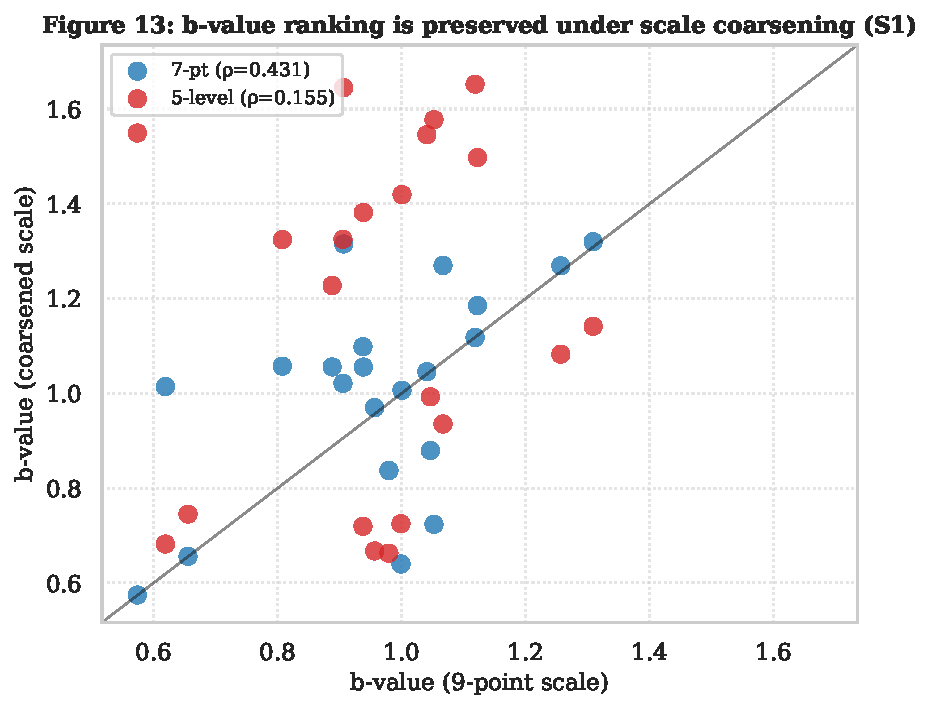
\includegraphics[width=0.7\linewidth]{fig13_scale_sensitivity.pdf}
\caption{S1: \sdi{} under scale coarsening. The 9-point grid is
load-bearing; both coarsenings fall well below the $\rho > 0.85$
stability threshold.}\label{fig:fig13}
\end{figure}

\begin{figure}[h]
\centering
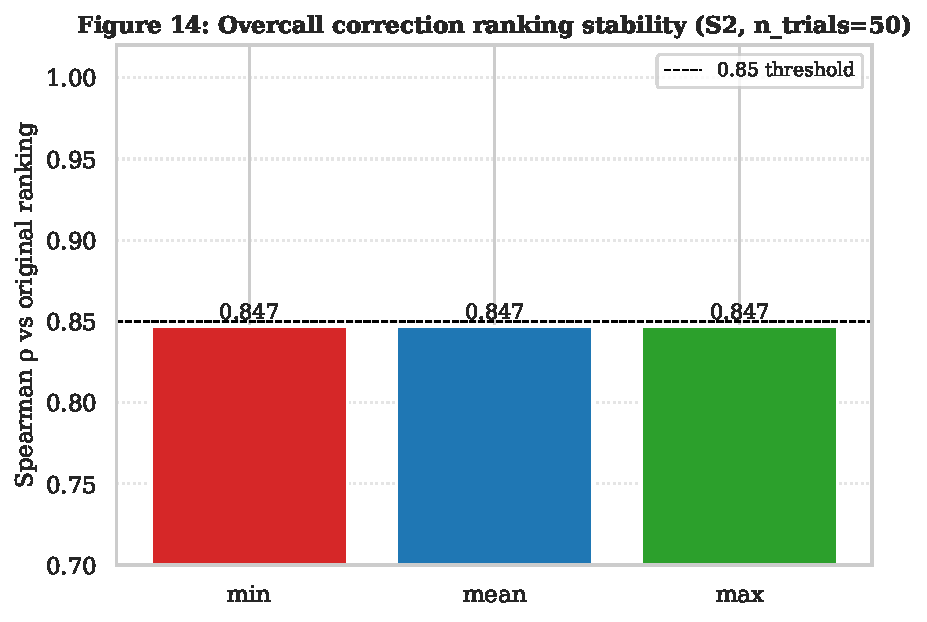
\includegraphics[width=0.7\linewidth]{fig14_overcall_sensitivity.pdf}
\caption{S2: ranking stability under overcall correction. Mean
Spearman $\rho = 0.847$ across $50$ bootstrap trials, narrowly
below the pre-registered $0.85$ threshold.}\label{fig:fig14}
\end{figure}

\begin{figure}[h]
\centering
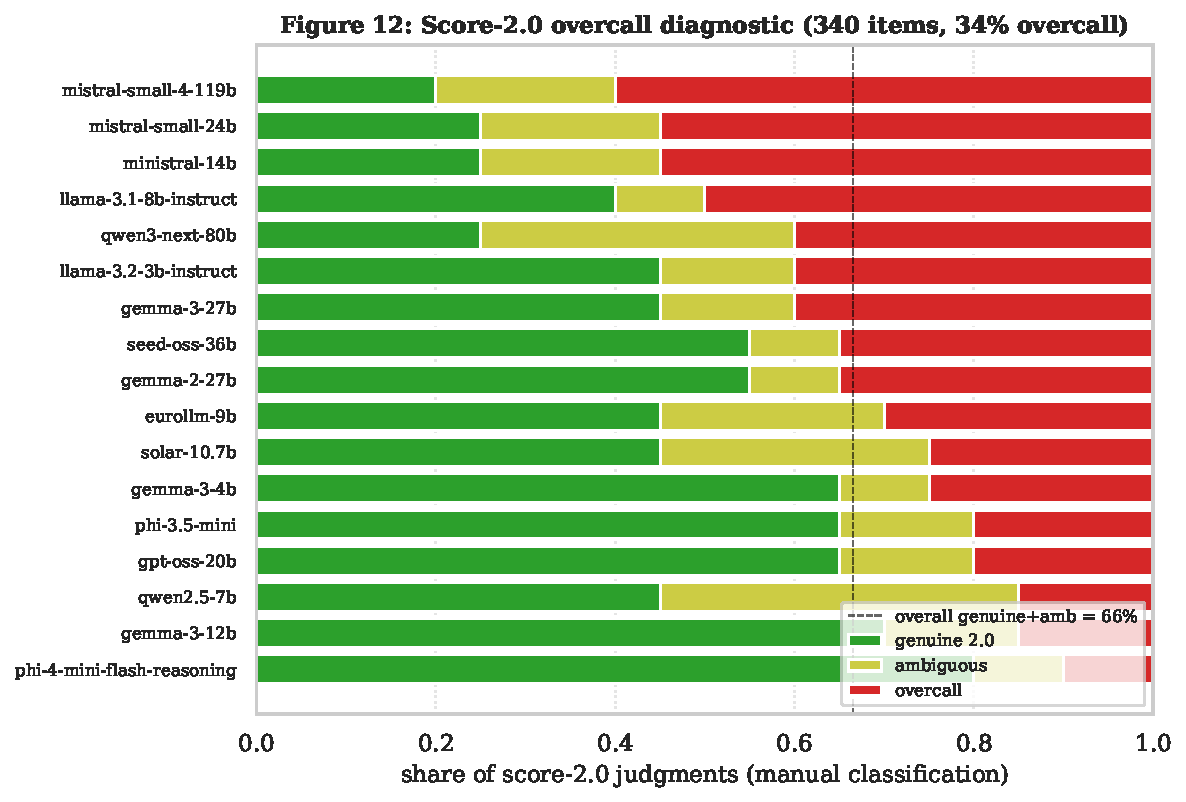
\includegraphics[width=0.85\linewidth]{fig12_overcall.pdf}
\caption{Per-model overcall breakdown on the $340$-item
human-rated subset (Appendix~\ref{app:overcall}).}\label{fig:fig12}
\end{figure}

\end{document}
